% Created by tikzDevice version 0.7.0 on 2014-06-29 19:47:57
% !TEX encoding = UTF-8 Unicode
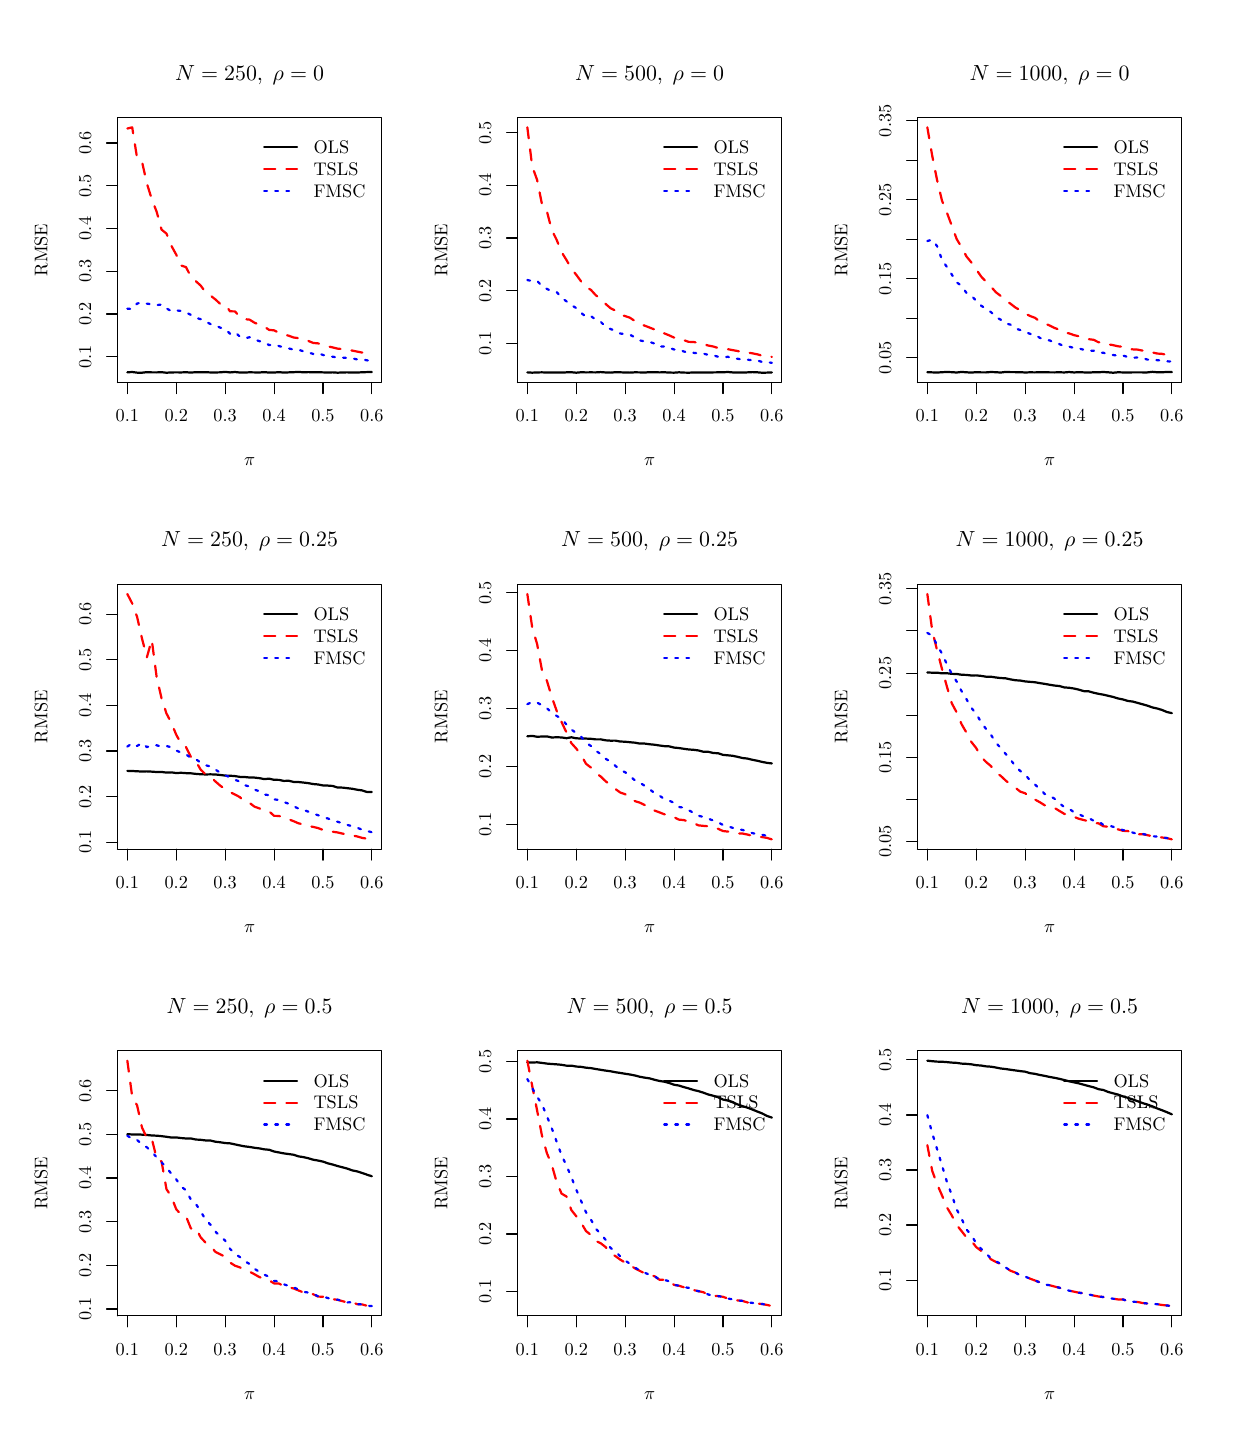
\begin{tikzpicture}[x=1pt,y=1pt]
\definecolor[named]{fillColor}{rgb}{1.00,1.00,1.00}
\path[use as bounding box,fill=fillColor,fill opacity=0.00] (0,0) rectangle (433.62,505.89);
\begin{scope}
\path[clip] ( 32.47,377.65) rectangle (127.91,473.42);
\definecolor[named]{drawColor}{rgb}{0.00,0.00,0.00}

\path[draw=drawColor,line width= 0.8pt,line join=round,line cap=round] ( 36.01,381.34) --
	( 37.77,381.46) --
	( 39.54,381.23) --
	( 41.31,381.21) --
	( 43.08,381.41) --
	( 44.84,381.33) --
	( 46.61,381.32) --
	( 48.38,381.39) --
	( 50.15,381.20) --
	( 51.91,381.31) --
	( 53.68,381.33) --
	( 55.45,381.31) --
	( 57.21,381.37) --
	( 58.98,381.27) --
	( 60.75,381.38) --
	( 62.52,381.35) --
	( 64.28,381.38) --
	( 66.05,381.31) --
	( 67.82,381.30) --
	( 69.59,381.34) --
	( 71.35,381.51) --
	( 73.12,381.31) --
	( 74.89,381.46) --
	( 76.66,381.28) --
	( 78.42,381.28) --
	( 80.19,381.35) --
	( 81.96,381.32) --
	( 83.72,381.29) --
	( 85.49,381.41) --
	( 87.26,381.26) --
	( 89.03,381.27) --
	( 90.79,381.40) --
	( 92.56,381.26) --
	( 94.33,381.33) --
	( 96.10,381.40) --
	( 97.86,381.48) --
	( 99.63,381.36) --
	(101.40,381.42) --
	(103.17,381.36) --
	(104.93,381.36) --
	(106.70,381.33) --
	(108.47,381.26) --
	(110.23,381.33) --
	(112.00,381.21) --
	(113.77,381.30) --
	(115.54,381.33) --
	(117.30,381.25) --
	(119.07,381.28) --
	(120.84,381.36) --
	(122.61,381.43) --
	(124.37,381.45);
\end{scope}
\begin{scope}
\path[clip] (  0.00,  0.00) rectangle (433.62,505.89);
\definecolor[named]{drawColor}{rgb}{0.00,0.00,0.00}

\path[draw=drawColor,line width= 0.4pt,line join=round,line cap=round] ( 36.01,377.65) -- (124.37,377.65);

\path[draw=drawColor,line width= 0.4pt,line join=round,line cap=round] ( 36.01,377.65) -- ( 36.01,373.69);

\path[draw=drawColor,line width= 0.4pt,line join=round,line cap=round] ( 53.68,377.65) -- ( 53.68,373.69);

\path[draw=drawColor,line width= 0.4pt,line join=round,line cap=round] ( 71.35,377.65) -- ( 71.35,373.69);

\path[draw=drawColor,line width= 0.4pt,line join=round,line cap=round] ( 89.03,377.65) -- ( 89.03,373.69);

\path[draw=drawColor,line width= 0.4pt,line join=round,line cap=round] (106.70,377.65) -- (106.70,373.69);

\path[draw=drawColor,line width= 0.4pt,line join=round,line cap=round] (124.37,377.65) -- (124.37,373.69);

\node[text=drawColor,anchor=base,inner sep=0pt, outer sep=0pt, scale=  0.66] at ( 36.01,363.40) {0.1};

\node[text=drawColor,anchor=base,inner sep=0pt, outer sep=0pt, scale=  0.66] at ( 53.68,363.40) {0.2};

\node[text=drawColor,anchor=base,inner sep=0pt, outer sep=0pt, scale=  0.66] at ( 71.35,363.40) {0.3};

\node[text=drawColor,anchor=base,inner sep=0pt, outer sep=0pt, scale=  0.66] at ( 89.03,363.40) {0.4};

\node[text=drawColor,anchor=base,inner sep=0pt, outer sep=0pt, scale=  0.66] at (106.70,363.40) {0.5};

\node[text=drawColor,anchor=base,inner sep=0pt, outer sep=0pt, scale=  0.66] at (124.37,363.40) {0.6};

\path[draw=drawColor,line width= 0.4pt,line join=round,line cap=round] ( 32.47,386.97) -- ( 32.47,464.20);

\path[draw=drawColor,line width= 0.4pt,line join=round,line cap=round] ( 32.47,386.97) -- ( 28.51,386.97);

\path[draw=drawColor,line width= 0.4pt,line join=round,line cap=round] ( 32.47,402.42) -- ( 28.51,402.42);

\path[draw=drawColor,line width= 0.4pt,line join=round,line cap=round] ( 32.47,417.86) -- ( 28.51,417.86);

\path[draw=drawColor,line width= 0.4pt,line join=round,line cap=round] ( 32.47,433.31) -- ( 28.51,433.31);

\path[draw=drawColor,line width= 0.4pt,line join=round,line cap=round] ( 32.47,448.76) -- ( 28.51,448.76);

\path[draw=drawColor,line width= 0.4pt,line join=round,line cap=round] ( 32.47,464.20) -- ( 28.51,464.20);

\node[text=drawColor,rotate= 90.00,anchor=base,inner sep=0pt, outer sep=0pt, scale=  0.66] at ( 22.97,386.97) {0.1};

\node[text=drawColor,rotate= 90.00,anchor=base,inner sep=0pt, outer sep=0pt, scale=  0.66] at ( 22.97,402.42) {0.2};

\node[text=drawColor,rotate= 90.00,anchor=base,inner sep=0pt, outer sep=0pt, scale=  0.66] at ( 22.97,417.86) {0.3};

\node[text=drawColor,rotate= 90.00,anchor=base,inner sep=0pt, outer sep=0pt, scale=  0.66] at ( 22.97,433.31) {0.4};

\node[text=drawColor,rotate= 90.00,anchor=base,inner sep=0pt, outer sep=0pt, scale=  0.66] at ( 22.97,448.76) {0.5};

\node[text=drawColor,rotate= 90.00,anchor=base,inner sep=0pt, outer sep=0pt, scale=  0.66] at ( 22.97,464.20) {0.6};

\path[draw=drawColor,line width= 0.4pt,line join=round,line cap=round] ( 32.47,377.65) --
	(127.91,377.65) --
	(127.91,473.42) --
	( 32.47,473.42) --
	( 32.47,377.65);
\end{scope}
\begin{scope}
\path[clip] (  0.00,337.26) rectangle (144.54,505.89);
\definecolor[named]{drawColor}{rgb}{0.00,0.00,0.00}

\node[text=drawColor,anchor=base,inner sep=0pt, outer sep=0pt, scale=  0.79] at ( 80.19,486.92) {\bfseries $N=250, \;\rho=0$};

\node[text=drawColor,anchor=base,inner sep=0pt, outer sep=0pt, scale=  0.66] at ( 80.19,347.56) {$\pi$};

\node[text=drawColor,rotate= 90.00,anchor=base,inner sep=0pt, outer sep=0pt, scale=  0.66] at (  7.13,425.53) {RMSE};
\end{scope}
\begin{scope}
\path[clip] ( 32.47,377.65) rectangle (127.91,473.42);
\definecolor[named]{drawColor}{rgb}{1.00,0.00,0.00}

\path[draw=drawColor,line width= 0.8pt,dash pattern=on 4pt off 4pt ,line join=round,line cap=round] ( 36.01,469.44) --
	( 37.77,469.87) --
	( 39.54,458.78) --
	( 41.31,457.47) --
	( 43.08,449.56) --
	( 44.84,443.92) --
	( 46.61,439.37) --
	( 48.38,432.91) --
	( 50.15,431.49) --
	( 51.91,427.10) --
	( 53.68,423.87) --
	( 55.45,419.93) --
	( 57.21,419.37) --
	( 58.98,415.90) --
	( 60.75,414.28) --
	( 62.52,412.69) --
	( 64.28,410.27) --
	( 66.05,409.09) --
	( 67.82,407.70) --
	( 69.59,406.05) --
	( 71.35,405.93) --
	( 73.12,403.38) --
	( 74.89,403.37) --
	( 76.66,401.43) --
	( 78.42,400.56) --
	( 80.19,400.38) --
	( 81.96,399.27) --
	( 83.72,398.57) --
	( 85.49,397.85) --
	( 87.26,396.68) --
	( 89.03,396.51) --
	( 90.79,395.66) --
	( 92.56,395.05) --
	( 94.33,394.57) --
	( 96.10,393.92) --
	( 97.86,393.70) --
	( 99.63,393.12) --
	(101.40,392.68) --
	(103.17,391.97) --
	(104.93,391.80) --
	(106.70,391.31) --
	(108.47,390.74) --
	(110.23,390.34) --
	(112.00,389.90) --
	(113.77,389.74) --
	(115.54,389.53) --
	(117.30,389.20) --
	(119.07,388.83) --
	(120.84,388.49) --
	(122.61,388.21) --
	(124.37,387.87);
\definecolor[named]{drawColor}{rgb}{0.00,0.00,1.00}

\path[draw=drawColor,line width= 0.8pt,dash pattern=on 1pt off 3pt ,line join=round,line cap=round] ( 36.01,404.34) --
	( 37.77,404.22) --
	( 39.54,406.20) --
	( 41.31,406.56) --
	( 43.08,406.16) --
	( 44.84,405.93) --
	( 46.61,405.64) --
	( 48.38,405.84) --
	( 50.15,404.46) --
	( 51.91,403.43) --
	( 53.68,403.73) --
	( 55.45,403.52) --
	( 57.21,403.01) --
	( 58.98,402.09) --
	( 60.75,401.06) --
	( 62.52,400.54) --
	( 64.28,399.69) --
	( 66.05,398.78) --
	( 67.82,398.27) --
	( 69.59,397.49) --
	( 71.35,396.97) --
	( 73.12,395.29) --
	( 74.89,395.88) --
	( 76.66,394.24) --
	( 78.42,393.64) --
	( 80.19,394.02) --
	( 81.96,393.25) --
	( 83.72,392.60) --
	( 85.49,392.23) --
	( 87.26,391.17) --
	( 89.03,391.29) --
	( 90.79,390.85) --
	( 92.56,390.31) --
	( 94.33,389.98) --
	( 96.10,389.55) --
	( 97.86,389.49) --
	( 99.63,388.96) --
	(101.40,388.54) --
	(103.17,387.99) --
	(104.93,388.29) --
	(106.70,387.62) --
	(108.47,387.21) --
	(110.23,386.98) --
	(112.00,386.67) --
	(113.77,386.66) --
	(115.54,386.53) --
	(117.30,386.37) --
	(119.07,386.01) --
	(120.84,386.00) --
	(122.61,385.68) --
	(124.37,385.43);
\definecolor[named]{drawColor}{rgb}{0.00,0.00,0.00}

\path[draw=drawColor,line width= 0.8pt,line join=round,line cap=round] ( 85.47,462.63) -- ( 97.35,462.63);
\definecolor[named]{drawColor}{rgb}{1.00,0.00,0.00}

\path[draw=drawColor,line width= 0.8pt,dash pattern=on 4pt off 4pt ,line join=round,line cap=round] ( 85.47,454.71) -- ( 97.35,454.71);
\definecolor[named]{drawColor}{rgb}{0.00,0.00,1.00}

\path[draw=drawColor,line width= 0.8pt,dash pattern=on 1pt off 3pt ,line join=round,line cap=round] ( 85.47,446.79) -- ( 97.35,446.79);
\definecolor[named]{drawColor}{rgb}{0.00,0.00,0.00}

\node[text=drawColor,anchor=base west,inner sep=0pt, outer sep=0pt, scale=  0.66] at (103.29,460.35) {OLS};

\node[text=drawColor,anchor=base west,inner sep=0pt, outer sep=0pt, scale=  0.66] at (103.29,452.43) {TSLS};

\node[text=drawColor,anchor=base west,inner sep=0pt, outer sep=0pt, scale=  0.66] at (103.29,444.51) {FMSC};
\end{scope}
\begin{scope}
\path[clip] (177.01,377.65) rectangle (272.45,473.42);
\definecolor[named]{drawColor}{rgb}{0.00,0.00,0.00}

\path[draw=drawColor,line width= 0.8pt,line join=round,line cap=round] (180.55,381.33) --
	(182.31,381.22) --
	(184.08,381.30) --
	(185.85,381.34) --
	(187.62,381.27) --
	(189.38,381.28) --
	(191.15,381.31) --
	(192.92,381.24) --
	(194.69,381.34) --
	(196.45,381.37) --
	(198.22,381.21) --
	(199.99,381.37) --
	(201.75,381.32) --
	(203.52,381.34) --
	(205.29,381.32) --
	(207.06,381.43) --
	(208.82,381.30) --
	(210.59,381.24) --
	(212.36,381.38) --
	(214.13,381.35) --
	(215.89,381.28) --
	(217.66,381.24) --
	(219.43,381.35) --
	(221.20,381.32) --
	(222.96,381.27) --
	(224.73,381.41) --
	(226.50,381.41) --
	(228.26,381.32) --
	(230.03,381.37) --
	(231.80,381.26) --
	(233.57,381.22) --
	(235.33,381.35) --
	(237.10,381.25) --
	(238.87,381.21) --
	(240.64,381.29) --
	(242.40,381.30) --
	(244.17,381.31) --
	(245.94,381.27) --
	(247.71,381.32) --
	(249.47,381.34) --
	(251.24,381.36) --
	(253.01,381.46) --
	(254.77,381.31) --
	(256.54,381.32) --
	(258.31,381.24) --
	(260.08,381.33) --
	(261.84,381.42) --
	(263.61,381.35) --
	(265.38,381.20) --
	(267.15,381.24) --
	(268.91,381.30);
\end{scope}
\begin{scope}
\path[clip] (  0.00,  0.00) rectangle (433.62,505.89);
\definecolor[named]{drawColor}{rgb}{0.00,0.00,0.00}

\path[draw=drawColor,line width= 0.4pt,line join=round,line cap=round] (180.55,377.65) -- (268.91,377.65);

\path[draw=drawColor,line width= 0.4pt,line join=round,line cap=round] (180.55,377.65) -- (180.55,373.69);

\path[draw=drawColor,line width= 0.4pt,line join=round,line cap=round] (198.22,377.65) -- (198.22,373.69);

\path[draw=drawColor,line width= 0.4pt,line join=round,line cap=round] (215.89,377.65) -- (215.89,373.69);

\path[draw=drawColor,line width= 0.4pt,line join=round,line cap=round] (233.57,377.65) -- (233.57,373.69);

\path[draw=drawColor,line width= 0.4pt,line join=round,line cap=round] (251.24,377.65) -- (251.24,373.69);

\path[draw=drawColor,line width= 0.4pt,line join=round,line cap=round] (268.91,377.65) -- (268.91,373.69);

\node[text=drawColor,anchor=base,inner sep=0pt, outer sep=0pt, scale=  0.66] at (180.55,363.40) {0.1};

\node[text=drawColor,anchor=base,inner sep=0pt, outer sep=0pt, scale=  0.66] at (198.22,363.40) {0.2};

\node[text=drawColor,anchor=base,inner sep=0pt, outer sep=0pt, scale=  0.66] at (215.89,363.40) {0.3};

\node[text=drawColor,anchor=base,inner sep=0pt, outer sep=0pt, scale=  0.66] at (233.57,363.40) {0.4};

\node[text=drawColor,anchor=base,inner sep=0pt, outer sep=0pt, scale=  0.66] at (251.24,363.40) {0.5};

\node[text=drawColor,anchor=base,inner sep=0pt, outer sep=0pt, scale=  0.66] at (268.91,363.40) {0.6};

\path[draw=drawColor,line width= 0.4pt,line join=round,line cap=round] (177.01,391.82) -- (177.01,467.98);

\path[draw=drawColor,line width= 0.4pt,line join=round,line cap=round] (177.01,391.82) -- (173.05,391.82);

\path[draw=drawColor,line width= 0.4pt,line join=round,line cap=round] (177.01,410.86) -- (173.05,410.86);

\path[draw=drawColor,line width= 0.4pt,line join=round,line cap=round] (177.01,429.90) -- (173.05,429.90);

\path[draw=drawColor,line width= 0.4pt,line join=round,line cap=round] (177.01,448.94) -- (173.05,448.94);

\path[draw=drawColor,line width= 0.4pt,line join=round,line cap=round] (177.01,467.98) -- (173.05,467.98);

\node[text=drawColor,rotate= 90.00,anchor=base,inner sep=0pt, outer sep=0pt, scale=  0.66] at (167.51,391.82) {0.1};

\node[text=drawColor,rotate= 90.00,anchor=base,inner sep=0pt, outer sep=0pt, scale=  0.66] at (167.51,410.86) {0.2};

\node[text=drawColor,rotate= 90.00,anchor=base,inner sep=0pt, outer sep=0pt, scale=  0.66] at (167.51,429.90) {0.3};

\node[text=drawColor,rotate= 90.00,anchor=base,inner sep=0pt, outer sep=0pt, scale=  0.66] at (167.51,448.94) {0.4};

\node[text=drawColor,rotate= 90.00,anchor=base,inner sep=0pt, outer sep=0pt, scale=  0.66] at (167.51,467.98) {0.5};

\path[draw=drawColor,line width= 0.4pt,line join=round,line cap=round] (177.01,377.65) --
	(272.45,377.65) --
	(272.45,473.42) --
	(177.01,473.42) --
	(177.01,377.65);
\end{scope}
\begin{scope}
\path[clip] (144.54,337.26) rectangle (289.08,505.89);
\definecolor[named]{drawColor}{rgb}{0.00,0.00,0.00}

\node[text=drawColor,anchor=base,inner sep=0pt, outer sep=0pt, scale=  0.79] at (224.73,486.92) {\bfseries $N=500, \;\rho=0$};

\node[text=drawColor,anchor=base,inner sep=0pt, outer sep=0pt, scale=  0.66] at (224.73,347.56) {$\pi$};

\node[text=drawColor,rotate= 90.00,anchor=base,inner sep=0pt, outer sep=0pt, scale=  0.66] at (151.67,425.53) {RMSE};
\end{scope}
\begin{scope}
\path[clip] (177.01,377.65) rectangle (272.45,473.42);
\definecolor[named]{drawColor}{rgb}{1.00,0.00,0.00}

\path[draw=drawColor,line width= 0.8pt,dash pattern=on 4pt off 4pt ,line join=round,line cap=round] (180.55,469.87) --
	(182.31,455.78) --
	(184.08,450.88) --
	(185.85,442.02) --
	(187.62,439.53) --
	(189.38,432.75) --
	(191.15,429.22) --
	(192.92,424.80) --
	(194.69,421.94) --
	(196.45,418.83) --
	(198.22,416.61) --
	(199.99,414.18) --
	(201.75,412.15) --
	(203.52,411.14) --
	(205.29,409.20) --
	(207.06,407.81) --
	(208.82,406.07) --
	(210.59,404.54) --
	(212.36,403.65) --
	(214.13,402.26) --
	(215.89,401.66) --
	(217.66,401.06) --
	(219.43,399.86) --
	(221.20,398.81) --
	(222.96,398.21) --
	(224.73,397.52) --
	(226.50,396.83) --
	(228.26,395.72) --
	(230.03,395.43) --
	(231.80,394.71) --
	(233.57,393.90) --
	(235.33,393.67) --
	(237.10,392.97) --
	(238.87,392.35) --
	(240.64,392.32) --
	(242.40,391.89) --
	(244.17,391.53) --
	(245.94,391.02) --
	(247.71,390.68) --
	(249.47,390.14) --
	(251.24,389.90) --
	(253.01,389.71) --
	(254.77,389.36) --
	(256.54,389.05) --
	(258.31,388.55) --
	(260.08,388.51) --
	(261.84,388.22) --
	(263.61,387.87) --
	(265.38,387.36) --
	(267.15,387.28) --
	(268.91,386.92);
\definecolor[named]{drawColor}{rgb}{0.00,0.00,1.00}

\path[draw=drawColor,line width= 0.8pt,dash pattern=on 1pt off 3pt ,line join=round,line cap=round] (180.55,414.69) --
	(182.31,414.33) --
	(184.08,414.40) --
	(185.85,412.51) --
	(187.62,411.49) --
	(189.38,410.64) --
	(191.15,410.37) --
	(192.92,408.29) --
	(194.69,407.00) --
	(196.45,405.61) --
	(198.22,404.58) --
	(199.99,402.84) --
	(201.75,401.39) --
	(203.52,401.65) --
	(205.29,400.39) --
	(207.06,399.58) --
	(208.82,397.89) --
	(210.59,397.01) --
	(212.36,396.31) --
	(214.13,395.38) --
	(215.89,395.11) --
	(217.66,394.92) --
	(219.43,393.95) --
	(221.20,392.86) --
	(222.96,392.54) --
	(224.73,392.32) --
	(226.50,391.75) --
	(228.26,390.61) --
	(230.03,390.72) --
	(231.80,390.17) --
	(233.57,389.61) --
	(235.33,389.54) --
	(237.10,388.88) --
	(238.87,388.36) --
	(240.64,388.39) --
	(242.40,388.20) --
	(244.17,388.11) --
	(245.94,387.64) --
	(247.71,387.47) --
	(249.47,386.98) --
	(251.24,386.79) --
	(253.01,386.96) --
	(254.77,386.42) --
	(256.54,386.26) --
	(258.31,385.89) --
	(260.08,385.90) --
	(261.84,385.73) --
	(263.61,385.64) --
	(265.38,385.08) --
	(267.15,385.01) --
	(268.91,384.78);
\definecolor[named]{drawColor}{rgb}{0.00,0.00,0.00}

\path[draw=drawColor,line width= 0.8pt,line join=round,line cap=round] (230.01,462.63) -- (241.89,462.63);
\definecolor[named]{drawColor}{rgb}{1.00,0.00,0.00}

\path[draw=drawColor,line width= 0.8pt,dash pattern=on 4pt off 4pt ,line join=round,line cap=round] (230.01,454.71) -- (241.89,454.71);
\definecolor[named]{drawColor}{rgb}{0.00,0.00,1.00}

\path[draw=drawColor,line width= 0.8pt,dash pattern=on 1pt off 3pt ,line join=round,line cap=round] (230.01,446.79) -- (241.89,446.79);
\definecolor[named]{drawColor}{rgb}{0.00,0.00,0.00}

\node[text=drawColor,anchor=base west,inner sep=0pt, outer sep=0pt, scale=  0.66] at (247.83,460.35) {OLS};

\node[text=drawColor,anchor=base west,inner sep=0pt, outer sep=0pt, scale=  0.66] at (247.83,452.43) {TSLS};

\node[text=drawColor,anchor=base west,inner sep=0pt, outer sep=0pt, scale=  0.66] at (247.83,444.51) {FMSC};
\end{scope}
\begin{scope}
\path[clip] (321.55,377.65) rectangle (416.99,473.42);
\definecolor[named]{drawColor}{rgb}{0.00,0.00,0.00}

\path[draw=drawColor,line width= 0.8pt,line join=round,line cap=round] (325.09,381.39) --
	(326.85,381.33) --
	(328.62,381.26) --
	(330.39,381.39) --
	(332.16,381.47) --
	(333.92,381.40) --
	(335.69,381.28) --
	(337.46,381.48) --
	(339.23,381.36) --
	(340.99,381.25) --
	(342.76,381.41) --
	(344.53,381.33) --
	(346.29,381.32) --
	(348.06,381.46) --
	(349.83,381.39) --
	(351.60,381.27) --
	(353.36,381.49) --
	(355.13,381.42) --
	(356.90,381.41) --
	(358.67,381.39) --
	(360.43,381.29) --
	(362.20,381.35) --
	(363.97,381.32) --
	(365.74,381.39) --
	(367.50,381.41) --
	(369.27,381.33) --
	(371.04,381.32) --
	(372.80,381.37) --
	(374.57,381.30) --
	(376.34,381.45) --
	(378.11,381.30) --
	(379.87,381.41) --
	(381.64,381.32) --
	(383.41,381.25) --
	(385.18,381.37) --
	(386.94,381.37) --
	(388.71,381.46) --
	(390.48,381.35) --
	(392.25,381.20) --
	(394.01,381.36) --
	(395.78,381.31) --
	(397.55,381.28) --
	(399.31,381.33) --
	(401.08,381.33) --
	(402.85,381.32) --
	(404.62,381.32) --
	(406.38,381.52) --
	(408.15,381.37) --
	(409.92,381.37) --
	(411.69,381.47) --
	(413.45,381.43);
\end{scope}
\begin{scope}
\path[clip] (  0.00,  0.00) rectangle (433.62,505.89);
\definecolor[named]{drawColor}{rgb}{0.00,0.00,0.00}

\path[draw=drawColor,line width= 0.4pt,line join=round,line cap=round] (325.09,377.65) -- (413.45,377.65);

\path[draw=drawColor,line width= 0.4pt,line join=round,line cap=round] (325.09,377.65) -- (325.09,373.69);

\path[draw=drawColor,line width= 0.4pt,line join=round,line cap=round] (342.76,377.65) -- (342.76,373.69);

\path[draw=drawColor,line width= 0.4pt,line join=round,line cap=round] (360.43,377.65) -- (360.43,373.69);

\path[draw=drawColor,line width= 0.4pt,line join=round,line cap=round] (378.11,377.65) -- (378.11,373.69);

\path[draw=drawColor,line width= 0.4pt,line join=round,line cap=round] (395.78,377.65) -- (395.78,373.69);

\path[draw=drawColor,line width= 0.4pt,line join=round,line cap=round] (413.45,377.65) -- (413.45,373.69);

\node[text=drawColor,anchor=base,inner sep=0pt, outer sep=0pt, scale=  0.66] at (325.09,363.40) {0.1};

\node[text=drawColor,anchor=base,inner sep=0pt, outer sep=0pt, scale=  0.66] at (342.76,363.40) {0.2};

\node[text=drawColor,anchor=base,inner sep=0pt, outer sep=0pt, scale=  0.66] at (360.43,363.40) {0.3};

\node[text=drawColor,anchor=base,inner sep=0pt, outer sep=0pt, scale=  0.66] at (378.11,363.40) {0.4};

\node[text=drawColor,anchor=base,inner sep=0pt, outer sep=0pt, scale=  0.66] at (395.78,363.40) {0.5};

\node[text=drawColor,anchor=base,inner sep=0pt, outer sep=0pt, scale=  0.66] at (413.45,363.40) {0.6};

\path[draw=drawColor,line width= 0.4pt,line join=round,line cap=round] (321.55,386.61) -- (321.55,472.22);

\path[draw=drawColor,line width= 0.4pt,line join=round,line cap=round] (321.55,386.61) -- (317.59,386.61);

\path[draw=drawColor,line width= 0.4pt,line join=round,line cap=round] (321.55,400.87) -- (317.59,400.87);

\path[draw=drawColor,line width= 0.4pt,line join=round,line cap=round] (321.55,415.14) -- (317.59,415.14);

\path[draw=drawColor,line width= 0.4pt,line join=round,line cap=round] (321.55,429.41) -- (317.59,429.41);

\path[draw=drawColor,line width= 0.4pt,line join=round,line cap=round] (321.55,443.68) -- (317.59,443.68);

\path[draw=drawColor,line width= 0.4pt,line join=round,line cap=round] (321.55,457.95) -- (317.59,457.95);

\path[draw=drawColor,line width= 0.4pt,line join=round,line cap=round] (321.55,472.22) -- (317.59,472.22);

\node[text=drawColor,rotate= 90.00,anchor=base,inner sep=0pt, outer sep=0pt, scale=  0.66] at (312.05,386.61) {0.05};

\node[text=drawColor,rotate= 90.00,anchor=base,inner sep=0pt, outer sep=0pt, scale=  0.66] at (312.05,415.14) {0.15};

\node[text=drawColor,rotate= 90.00,anchor=base,inner sep=0pt, outer sep=0pt, scale=  0.66] at (312.05,443.68) {0.25};

\node[text=drawColor,rotate= 90.00,anchor=base,inner sep=0pt, outer sep=0pt, scale=  0.66] at (312.05,472.22) {0.35};

\path[draw=drawColor,line width= 0.4pt,line join=round,line cap=round] (321.55,377.65) --
	(416.99,377.65) --
	(416.99,473.42) --
	(321.55,473.42) --
	(321.55,377.65);
\end{scope}
\begin{scope}
\path[clip] (289.08,337.26) rectangle (433.62,505.89);
\definecolor[named]{drawColor}{rgb}{0.00,0.00,0.00}

\node[text=drawColor,anchor=base,inner sep=0pt, outer sep=0pt, scale=  0.79] at (369.27,486.92) {\bfseries $N=1000, \;\rho=0$};

\node[text=drawColor,anchor=base,inner sep=0pt, outer sep=0pt, scale=  0.66] at (369.27,347.56) {$\pi$};

\node[text=drawColor,rotate= 90.00,anchor=base,inner sep=0pt, outer sep=0pt, scale=  0.66] at (296.21,425.53) {RMSE};
\end{scope}
\begin{scope}
\path[clip] (321.55,377.65) rectangle (416.99,473.42);
\definecolor[named]{drawColor}{rgb}{1.00,0.00,0.00}

\path[draw=drawColor,line width= 0.8pt,dash pattern=on 4pt off 4pt ,line join=round,line cap=round] (325.09,469.87) --
	(326.85,459.63) --
	(328.62,450.78) --
	(330.39,443.37) --
	(332.16,439.04) --
	(333.92,434.34) --
	(335.69,429.51) --
	(337.46,426.56) --
	(339.23,423.21) --
	(340.99,421.06) --
	(342.76,418.56) --
	(344.53,415.96) --
	(346.29,414.11) --
	(348.06,412.32) --
	(349.83,410.32) --
	(351.60,408.93) --
	(353.36,407.38) --
	(355.13,406.14) --
	(356.90,404.76) --
	(358.67,403.78) --
	(360.43,402.62) --
	(362.20,401.70) --
	(363.97,401.05) --
	(365.74,399.71) --
	(367.50,399.02) --
	(369.27,398.26) --
	(371.04,397.38) --
	(372.80,396.74) --
	(374.57,395.77) --
	(376.34,395.41) --
	(378.11,394.78) --
	(379.87,394.36) --
	(381.64,393.88) --
	(383.41,393.32) --
	(385.18,393.10) --
	(386.94,392.21) --
	(388.71,392.17) --
	(390.48,391.48) --
	(392.25,391.15) --
	(394.01,390.75) --
	(395.78,390.55) --
	(397.55,389.87) --
	(399.31,389.64) --
	(401.08,389.55) --
	(402.85,389.20) --
	(404.62,388.69) --
	(406.38,388.55) --
	(408.15,388.13) --
	(409.92,388.02) --
	(411.69,387.62) --
	(413.45,387.57);
\definecolor[named]{drawColor}{rgb}{0.00,0.00,1.00}

\path[draw=drawColor,line width= 0.8pt,dash pattern=on 1pt off 3pt ,line join=round,line cap=round] (325.09,428.79) --
	(326.85,429.28) --
	(328.62,426.92) --
	(330.39,422.02) --
	(332.16,419.41) --
	(333.92,416.69) --
	(335.69,413.87) --
	(337.46,412.59) --
	(339.23,410.03) --
	(340.99,409.11) --
	(342.76,407.14) --
	(344.53,405.45) --
	(346.29,404.24) --
	(348.06,403.13) --
	(349.83,401.34) --
	(351.60,400.36) --
	(353.36,399.04) --
	(355.13,398.56) --
	(356.90,397.23) --
	(358.67,396.61) --
	(360.43,395.95) --
	(362.20,395.25) --
	(363.97,394.93) --
	(365.74,393.81) --
	(367.50,393.08) --
	(369.27,392.88) --
	(371.04,392.02) --
	(372.80,391.54) --
	(374.57,390.82) --
	(376.34,390.63) --
	(378.11,390.12) --
	(379.87,389.96) --
	(381.64,389.49) --
	(383.41,389.09) --
	(385.18,389.18) --
	(386.94,388.49) --
	(388.71,388.42) --
	(390.48,387.86) --
	(392.25,387.59) --
	(394.01,387.35) --
	(395.78,387.42) --
	(397.55,386.85) --
	(399.31,386.61) --
	(401.08,386.70) --
	(402.85,386.49) --
	(404.62,385.94) --
	(406.38,385.92) --
	(408.15,385.74) --
	(409.92,385.60) --
	(411.69,385.33) --
	(413.45,385.23);
\definecolor[named]{drawColor}{rgb}{0.00,0.00,0.00}

\path[draw=drawColor,line width= 0.8pt,line join=round,line cap=round] (374.55,462.63) -- (386.43,462.63);
\definecolor[named]{drawColor}{rgb}{1.00,0.00,0.00}

\path[draw=drawColor,line width= 0.8pt,dash pattern=on 4pt off 4pt ,line join=round,line cap=round] (374.55,454.71) -- (386.43,454.71);
\definecolor[named]{drawColor}{rgb}{0.00,0.00,1.00}

\path[draw=drawColor,line width= 0.8pt,dash pattern=on 1pt off 3pt ,line join=round,line cap=round] (374.55,446.79) -- (386.43,446.79);
\definecolor[named]{drawColor}{rgb}{0.00,0.00,0.00}

\node[text=drawColor,anchor=base west,inner sep=0pt, outer sep=0pt, scale=  0.66] at (392.37,460.35) {OLS};

\node[text=drawColor,anchor=base west,inner sep=0pt, outer sep=0pt, scale=  0.66] at (392.37,452.43) {TSLS};

\node[text=drawColor,anchor=base west,inner sep=0pt, outer sep=0pt, scale=  0.66] at (392.37,444.51) {FMSC};
\end{scope}
\begin{scope}
\path[clip] ( 32.47,209.02) rectangle (127.91,304.79);
\definecolor[named]{drawColor}{rgb}{0.00,0.00,0.00}

\path[draw=drawColor,line width= 0.8pt,line join=round,line cap=round] ( 36.01,237.33) --
	( 37.77,237.28) --
	( 39.54,237.19) --
	( 41.31,237.08) --
	( 43.08,237.15) --
	( 44.84,237.05) --
	( 46.61,236.92) --
	( 48.38,236.94) --
	( 50.15,236.71) --
	( 51.91,236.79) --
	( 53.68,236.55) --
	( 55.45,236.64) --
	( 57.21,236.51) --
	( 58.98,236.45) --
	( 60.75,236.24) --
	( 62.52,236.11) --
	( 64.28,236.04) --
	( 66.05,236.08) --
	( 67.82,236.03) --
	( 69.59,235.85) --
	( 71.35,235.63) --
	( 73.12,235.58) --
	( 74.89,235.45) --
	( 76.66,235.16) --
	( 78.42,235.11) --
	( 80.19,234.93) --
	( 81.96,234.90) --
	( 83.72,234.70) --
	( 85.49,234.37) --
	( 87.26,234.51) --
	( 89.03,234.10) --
	( 90.79,234.08) --
	( 92.56,233.70) --
	( 94.33,233.76) --
	( 96.10,233.34) --
	( 97.86,233.30) --
	( 99.63,233.11) --
	(101.40,232.90) --
	(103.17,232.57) --
	(104.93,232.42) --
	(106.70,232.06) --
	(108.47,232.01) --
	(110.23,231.88) --
	(112.00,231.31) --
	(113.77,231.28) --
	(115.54,231.07) --
	(117.30,230.86) --
	(119.07,230.51) --
	(120.84,230.28) --
	(122.61,229.70) --
	(124.37,229.70);
\end{scope}
\begin{scope}
\path[clip] (  0.00,  0.00) rectangle (433.62,505.89);
\definecolor[named]{drawColor}{rgb}{0.00,0.00,0.00}

\path[draw=drawColor,line width= 0.4pt,line join=round,line cap=round] ( 36.01,209.02) -- (124.37,209.02);

\path[draw=drawColor,line width= 0.4pt,line join=round,line cap=round] ( 36.01,209.02) -- ( 36.01,205.06);

\path[draw=drawColor,line width= 0.4pt,line join=round,line cap=round] ( 53.68,209.02) -- ( 53.68,205.06);

\path[draw=drawColor,line width= 0.4pt,line join=round,line cap=round] ( 71.35,209.02) -- ( 71.35,205.06);

\path[draw=drawColor,line width= 0.4pt,line join=round,line cap=round] ( 89.03,209.02) -- ( 89.03,205.06);

\path[draw=drawColor,line width= 0.4pt,line join=round,line cap=round] (106.70,209.02) -- (106.70,205.06);

\path[draw=drawColor,line width= 0.4pt,line join=round,line cap=round] (124.37,209.02) -- (124.37,205.06);

\node[text=drawColor,anchor=base,inner sep=0pt, outer sep=0pt, scale=  0.66] at ( 36.01,194.77) {0.1};

\node[text=drawColor,anchor=base,inner sep=0pt, outer sep=0pt, scale=  0.66] at ( 53.68,194.77) {0.2};

\node[text=drawColor,anchor=base,inner sep=0pt, outer sep=0pt, scale=  0.66] at ( 71.35,194.77) {0.3};

\node[text=drawColor,anchor=base,inner sep=0pt, outer sep=0pt, scale=  0.66] at ( 89.03,194.77) {0.4};

\node[text=drawColor,anchor=base,inner sep=0pt, outer sep=0pt, scale=  0.66] at (106.70,194.77) {0.5};

\node[text=drawColor,anchor=base,inner sep=0pt, outer sep=0pt, scale=  0.66] at (124.37,194.77) {0.6};

\path[draw=drawColor,line width= 0.4pt,line join=round,line cap=round] ( 32.47,211.55) -- ( 32.47,293.97);

\path[draw=drawColor,line width= 0.4pt,line join=round,line cap=round] ( 32.47,211.55) -- ( 28.51,211.55);

\path[draw=drawColor,line width= 0.4pt,line join=round,line cap=round] ( 32.47,228.04) -- ( 28.51,228.04);

\path[draw=drawColor,line width= 0.4pt,line join=round,line cap=round] ( 32.47,244.52) -- ( 28.51,244.52);

\path[draw=drawColor,line width= 0.4pt,line join=round,line cap=round] ( 32.47,261.01) -- ( 28.51,261.01);

\path[draw=drawColor,line width= 0.4pt,line join=round,line cap=round] ( 32.47,277.49) -- ( 28.51,277.49);

\path[draw=drawColor,line width= 0.4pt,line join=round,line cap=round] ( 32.47,293.97) -- ( 28.51,293.97);

\node[text=drawColor,rotate= 90.00,anchor=base,inner sep=0pt, outer sep=0pt, scale=  0.66] at ( 22.97,211.55) {0.1};

\node[text=drawColor,rotate= 90.00,anchor=base,inner sep=0pt, outer sep=0pt, scale=  0.66] at ( 22.97,228.04) {0.2};

\node[text=drawColor,rotate= 90.00,anchor=base,inner sep=0pt, outer sep=0pt, scale=  0.66] at ( 22.97,244.52) {0.3};

\node[text=drawColor,rotate= 90.00,anchor=base,inner sep=0pt, outer sep=0pt, scale=  0.66] at ( 22.97,261.01) {0.4};

\node[text=drawColor,rotate= 90.00,anchor=base,inner sep=0pt, outer sep=0pt, scale=  0.66] at ( 22.97,277.49) {0.5};

\node[text=drawColor,rotate= 90.00,anchor=base,inner sep=0pt, outer sep=0pt, scale=  0.66] at ( 22.97,293.97) {0.6};

\path[draw=drawColor,line width= 0.4pt,line join=round,line cap=round] ( 32.47,209.02) --
	(127.91,209.02) --
	(127.91,304.79) --
	( 32.47,304.79) --
	( 32.47,209.02);
\end{scope}
\begin{scope}
\path[clip] (  0.00,168.63) rectangle (144.54,337.26);
\definecolor[named]{drawColor}{rgb}{0.00,0.00,0.00}

\node[text=drawColor,anchor=base,inner sep=0pt, outer sep=0pt, scale=  0.79] at ( 80.19,318.29) {\bfseries $N=250, \;\rho=0.25$};

\node[text=drawColor,anchor=base,inner sep=0pt, outer sep=0pt, scale=  0.66] at ( 80.19,178.93) {$\pi$};

\node[text=drawColor,rotate= 90.00,anchor=base,inner sep=0pt, outer sep=0pt, scale=  0.66] at (  7.13,256.90) {RMSE};
\end{scope}
\begin{scope}
\path[clip] ( 32.47,209.02) rectangle (127.91,304.79);
\definecolor[named]{drawColor}{rgb}{1.00,0.00,0.00}

\path[draw=drawColor,line width= 0.8pt,dash pattern=on 4pt off 4pt ,line join=round,line cap=round] ( 36.01,301.24) --
	( 37.77,297.86) --
	( 39.54,292.97) --
	( 41.31,285.14) --
	( 43.08,278.39) --
	( 44.84,284.69) --
	( 46.61,271.15) --
	( 48.38,263.53) --
	( 50.15,258.08) --
	( 51.91,254.71) --
	( 53.68,250.39) --
	( 55.45,247.20) --
	( 57.21,245.92) --
	( 58.98,242.35) --
	( 60.75,240.80) --
	( 62.52,237.77) --
	( 64.28,236.06) --
	( 66.05,235.23) --
	( 67.82,233.52) --
	( 69.59,231.98) --
	( 71.35,230.72) --
	( 73.12,229.65) --
	( 74.89,228.80) --
	( 76.66,227.86) --
	( 78.42,226.10) --
	( 80.19,225.75) --
	( 81.96,224.40) --
	( 83.72,223.77) --
	( 85.49,222.93) --
	( 87.26,222.70) --
	( 89.03,221.08) --
	( 90.79,221.05) --
	( 92.56,220.41) --
	( 94.33,219.82) --
	( 96.10,219.15) --
	( 97.86,218.38) --
	( 99.63,217.97) --
	(101.40,217.40) --
	(103.17,217.09) --
	(104.93,216.66) --
	(106.70,216.00) --
	(108.47,215.76) --
	(110.23,215.34) --
	(112.00,215.08) --
	(113.77,214.66) --
	(115.54,214.31) --
	(117.30,214.00) --
	(119.07,213.64) --
	(120.84,213.12) --
	(122.61,212.83) --
	(124.37,212.57);
\definecolor[named]{drawColor}{rgb}{0.00,0.00,1.00}

\path[draw=drawColor,line width= 0.8pt,dash pattern=on 1pt off 3pt ,line join=round,line cap=round] ( 36.01,246.11) --
	( 37.77,247.27) --
	( 39.54,246.33) --
	( 41.31,247.43) --
	( 43.08,245.92) --
	( 44.84,246.59) --
	( 46.61,246.57) --
	( 48.38,246.08) --
	( 50.15,246.32) --
	( 51.91,245.84) --
	( 53.68,244.70) --
	( 55.45,243.90) --
	( 57.21,243.27) --
	( 58.98,242.06) --
	( 60.75,241.59) --
	( 62.52,240.28) --
	( 64.28,239.36) --
	( 66.05,238.93) --
	( 67.82,237.83) --
	( 69.59,236.64) --
	( 71.35,235.71) --
	( 73.12,235.06) --
	( 74.89,234.09) --
	( 76.66,233.49) --
	( 78.42,232.16) --
	( 80.19,231.65) --
	( 81.96,230.53) --
	( 83.72,229.99) --
	( 85.49,228.79) --
	( 87.26,228.55) --
	( 89.03,227.04) --
	( 90.79,226.82) --
	( 92.56,226.09) --
	( 94.33,225.45) --
	( 96.10,224.56) --
	( 97.86,223.69) --
	( 99.63,223.28) --
	(101.40,222.58) --
	(103.17,221.91) --
	(104.93,221.31) --
	(106.70,220.61) --
	(108.47,220.13) --
	(110.23,219.41) --
	(112.00,218.95) --
	(113.77,218.35) --
	(115.54,217.79) --
	(117.30,217.33) --
	(119.07,216.78) --
	(120.84,216.07) --
	(122.61,215.66) --
	(124.37,215.14);
\definecolor[named]{drawColor}{rgb}{0.00,0.00,0.00}

\path[draw=drawColor,line width= 0.8pt,line join=round,line cap=round] ( 85.47,294.00) -- ( 97.35,294.00);
\definecolor[named]{drawColor}{rgb}{1.00,0.00,0.00}

\path[draw=drawColor,line width= 0.8pt,dash pattern=on 4pt off 4pt ,line join=round,line cap=round] ( 85.47,286.08) -- ( 97.35,286.08);
\definecolor[named]{drawColor}{rgb}{0.00,0.00,1.00}

\path[draw=drawColor,line width= 0.8pt,dash pattern=on 1pt off 3pt ,line join=round,line cap=round] ( 85.47,278.16) -- ( 97.35,278.16);
\definecolor[named]{drawColor}{rgb}{0.00,0.00,0.00}

\node[text=drawColor,anchor=base west,inner sep=0pt, outer sep=0pt, scale=  0.66] at (103.29,291.72) {OLS};

\node[text=drawColor,anchor=base west,inner sep=0pt, outer sep=0pt, scale=  0.66] at (103.29,283.80) {TSLS};

\node[text=drawColor,anchor=base west,inner sep=0pt, outer sep=0pt, scale=  0.66] at (103.29,275.88) {FMSC};
\end{scope}
\begin{scope}
\path[clip] (177.01,209.02) rectangle (272.45,304.79);
\definecolor[named]{drawColor}{rgb}{0.00,0.00,0.00}

\path[draw=drawColor,line width= 0.8pt,line join=round,line cap=round] (180.55,249.83) --
	(182.31,249.97) --
	(184.08,249.66) --
	(185.85,249.74) --
	(187.62,249.79) --
	(189.38,249.39) --
	(191.15,249.48) --
	(192.92,249.41) --
	(194.69,249.14) --
	(196.45,249.47) --
	(198.22,249.10) --
	(199.99,249.03) --
	(201.75,249.00) --
	(203.52,248.92) --
	(205.29,248.71) --
	(207.06,248.72) --
	(208.82,248.37) --
	(210.59,248.25) --
	(212.36,248.26) --
	(214.13,247.94) --
	(215.89,247.86) --
	(217.66,247.68) --
	(219.43,247.52) --
	(221.20,247.19) --
	(222.96,247.19) --
	(224.73,246.95) --
	(226.50,246.78) --
	(228.26,246.51) --
	(230.03,246.27) --
	(231.80,246.19) --
	(233.57,245.75) --
	(235.33,245.58) --
	(237.10,245.31) --
	(238.87,245.06) --
	(240.64,244.94) --
	(242.40,244.71) --
	(244.17,244.24) --
	(245.94,244.23) --
	(247.71,243.79) --
	(249.47,243.70) --
	(251.24,243.12) --
	(253.01,242.95) --
	(254.77,242.78) --
	(256.54,242.40) --
	(258.31,241.97) --
	(260.08,241.78) --
	(261.84,241.34) --
	(263.61,241.00) --
	(265.38,240.57) --
	(267.15,240.23) --
	(268.91,240.02);
\end{scope}
\begin{scope}
\path[clip] (  0.00,  0.00) rectangle (433.62,505.89);
\definecolor[named]{drawColor}{rgb}{0.00,0.00,0.00}

\path[draw=drawColor,line width= 0.4pt,line join=round,line cap=round] (180.55,209.02) -- (268.91,209.02);

\path[draw=drawColor,line width= 0.4pt,line join=round,line cap=round] (180.55,209.02) -- (180.55,205.06);

\path[draw=drawColor,line width= 0.4pt,line join=round,line cap=round] (198.22,209.02) -- (198.22,205.06);

\path[draw=drawColor,line width= 0.4pt,line join=round,line cap=round] (215.89,209.02) -- (215.89,205.06);

\path[draw=drawColor,line width= 0.4pt,line join=round,line cap=round] (233.57,209.02) -- (233.57,205.06);

\path[draw=drawColor,line width= 0.4pt,line join=round,line cap=round] (251.24,209.02) -- (251.24,205.06);

\path[draw=drawColor,line width= 0.4pt,line join=round,line cap=round] (268.91,209.02) -- (268.91,205.06);

\node[text=drawColor,anchor=base,inner sep=0pt, outer sep=0pt, scale=  0.66] at (180.55,194.77) {0.1};

\node[text=drawColor,anchor=base,inner sep=0pt, outer sep=0pt, scale=  0.66] at (198.22,194.77) {0.2};

\node[text=drawColor,anchor=base,inner sep=0pt, outer sep=0pt, scale=  0.66] at (215.89,194.77) {0.3};

\node[text=drawColor,anchor=base,inner sep=0pt, outer sep=0pt, scale=  0.66] at (233.57,194.77) {0.4};

\node[text=drawColor,anchor=base,inner sep=0pt, outer sep=0pt, scale=  0.66] at (251.24,194.77) {0.5};

\node[text=drawColor,anchor=base,inner sep=0pt, outer sep=0pt, scale=  0.66] at (268.91,194.77) {0.6};

\path[draw=drawColor,line width= 0.4pt,line join=round,line cap=round] (177.01,217.97) -- (177.01,301.77);

\path[draw=drawColor,line width= 0.4pt,line join=round,line cap=round] (177.01,217.97) -- (173.05,217.97);

\path[draw=drawColor,line width= 0.4pt,line join=round,line cap=round] (177.01,238.92) -- (173.05,238.92);

\path[draw=drawColor,line width= 0.4pt,line join=round,line cap=round] (177.01,259.87) -- (173.05,259.87);

\path[draw=drawColor,line width= 0.4pt,line join=round,line cap=round] (177.01,280.82) -- (173.05,280.82);

\path[draw=drawColor,line width= 0.4pt,line join=round,line cap=round] (177.01,301.77) -- (173.05,301.77);

\node[text=drawColor,rotate= 90.00,anchor=base,inner sep=0pt, outer sep=0pt, scale=  0.66] at (167.51,217.97) {0.1};

\node[text=drawColor,rotate= 90.00,anchor=base,inner sep=0pt, outer sep=0pt, scale=  0.66] at (167.51,238.92) {0.2};

\node[text=drawColor,rotate= 90.00,anchor=base,inner sep=0pt, outer sep=0pt, scale=  0.66] at (167.51,259.87) {0.3};

\node[text=drawColor,rotate= 90.00,anchor=base,inner sep=0pt, outer sep=0pt, scale=  0.66] at (167.51,280.82) {0.4};

\node[text=drawColor,rotate= 90.00,anchor=base,inner sep=0pt, outer sep=0pt, scale=  0.66] at (167.51,301.77) {0.5};

\path[draw=drawColor,line width= 0.4pt,line join=round,line cap=round] (177.01,209.02) --
	(272.45,209.02) --
	(272.45,304.79) --
	(177.01,304.79) --
	(177.01,209.02);
\end{scope}
\begin{scope}
\path[clip] (144.54,168.63) rectangle (289.08,337.26);
\definecolor[named]{drawColor}{rgb}{0.00,0.00,0.00}

\node[text=drawColor,anchor=base,inner sep=0pt, outer sep=0pt, scale=  0.79] at (224.73,318.29) {\bfseries $N=500, \;\rho=0.25$};

\node[text=drawColor,anchor=base,inner sep=0pt, outer sep=0pt, scale=  0.66] at (224.73,178.93) {$\pi$};

\node[text=drawColor,rotate= 90.00,anchor=base,inner sep=0pt, outer sep=0pt, scale=  0.66] at (151.67,256.90) {RMSE};
\end{scope}
\begin{scope}
\path[clip] (177.01,209.02) rectangle (272.45,304.79);
\definecolor[named]{drawColor}{rgb}{1.00,0.00,0.00}

\path[draw=drawColor,line width= 0.8pt,dash pattern=on 4pt off 4pt ,line join=round,line cap=round] (180.55,301.24) --
	(182.31,289.15) --
	(184.08,283.18) --
	(185.85,273.61) --
	(187.62,269.89) --
	(189.38,264.06) --
	(191.15,259.03) --
	(192.92,254.97) --
	(194.69,251.21) --
	(196.45,247.36) --
	(198.22,245.40) --
	(199.99,243.05) --
	(201.75,239.91) --
	(203.52,238.52) --
	(205.29,236.54) --
	(207.06,235.30) --
	(208.82,233.59) --
	(210.59,232.25) --
	(212.36,230.78) --
	(214.13,229.51) --
	(215.89,228.90) --
	(217.66,227.44) --
	(219.43,226.41) --
	(221.20,225.84) --
	(222.96,225.00) --
	(224.73,224.02) --
	(226.50,223.00) --
	(228.26,222.35) --
	(230.03,221.66) --
	(231.80,221.32) --
	(233.57,220.60) --
	(235.33,219.72) --
	(237.10,219.55) --
	(238.87,218.98) --
	(240.64,218.46) --
	(242.40,217.64) --
	(244.17,217.46) --
	(245.94,217.32) --
	(247.71,216.79) --
	(249.47,216.41) --
	(251.24,215.59) --
	(253.01,215.40) --
	(254.77,215.07) --
	(256.54,214.71) --
	(258.31,214.69) --
	(260.08,214.32) --
	(261.84,213.88) --
	(263.61,213.49) --
	(265.38,213.40) --
	(267.15,213.11) --
	(268.91,212.57);
\definecolor[named]{drawColor}{rgb}{0.00,0.00,1.00}

\path[draw=drawColor,line width= 0.8pt,dash pattern=on 1pt off 3pt ,line join=round,line cap=round] (180.55,261.44) --
	(182.31,262.19) --
	(184.08,262.03) --
	(185.85,260.99) --
	(187.62,259.94) --
	(189.38,258.43) --
	(191.15,257.18) --
	(192.92,256.23) --
	(194.69,254.05) --
	(196.45,252.28) --
	(198.22,251.00) --
	(199.99,249.66) --
	(201.75,247.56) --
	(203.52,246.31) --
	(205.29,244.59) --
	(207.06,243.41) --
	(208.82,241.73) --
	(210.59,240.66) --
	(212.36,239.16) --
	(214.13,237.71) --
	(215.89,236.85) --
	(217.66,235.39) --
	(219.43,233.90) --
	(221.20,233.09) --
	(222.96,231.91) --
	(224.73,230.68) --
	(226.50,229.33) --
	(228.26,228.42) --
	(230.03,227.15) --
	(231.80,226.57) --
	(233.57,225.77) --
	(235.33,224.28) --
	(237.10,224.04) --
	(238.87,223.10) --
	(240.64,222.15) --
	(242.40,221.12) --
	(244.17,220.68) --
	(245.94,220.06) --
	(247.71,219.39) --
	(249.47,218.77) --
	(251.24,217.76) --
	(253.01,217.28) --
	(254.77,216.75) --
	(256.54,216.28) --
	(258.31,215.98) --
	(260.08,215.56) --
	(261.84,214.87) --
	(263.61,214.39) --
	(265.38,214.24) --
	(267.15,213.86) --
	(268.91,213.19);
\definecolor[named]{drawColor}{rgb}{0.00,0.00,0.00}

\path[draw=drawColor,line width= 0.8pt,line join=round,line cap=round] (230.01,294.00) -- (241.89,294.00);
\definecolor[named]{drawColor}{rgb}{1.00,0.00,0.00}

\path[draw=drawColor,line width= 0.8pt,dash pattern=on 4pt off 4pt ,line join=round,line cap=round] (230.01,286.08) -- (241.89,286.08);
\definecolor[named]{drawColor}{rgb}{0.00,0.00,1.00}

\path[draw=drawColor,line width= 0.8pt,dash pattern=on 1pt off 3pt ,line join=round,line cap=round] (230.01,278.16) -- (241.89,278.16);
\definecolor[named]{drawColor}{rgb}{0.00,0.00,0.00}

\node[text=drawColor,anchor=base west,inner sep=0pt, outer sep=0pt, scale=  0.66] at (247.83,291.72) {OLS};

\node[text=drawColor,anchor=base west,inner sep=0pt, outer sep=0pt, scale=  0.66] at (247.83,283.80) {TSLS};

\node[text=drawColor,anchor=base west,inner sep=0pt, outer sep=0pt, scale=  0.66] at (247.83,275.88) {FMSC};
\end{scope}
\begin{scope}
\path[clip] (321.55,209.02) rectangle (416.99,304.79);
\definecolor[named]{drawColor}{rgb}{0.00,0.00,0.00}

\path[draw=drawColor,line width= 0.8pt,line join=round,line cap=round] (325.09,272.89) --
	(326.85,272.81) --
	(328.62,272.82) --
	(330.39,272.57) --
	(332.16,272.61) --
	(333.92,272.39) --
	(335.69,272.34) --
	(337.46,272.07) --
	(339.23,272.00) --
	(340.99,271.80) --
	(342.76,271.84) --
	(344.53,271.65) --
	(346.29,271.36) --
	(348.06,271.36) --
	(349.83,271.08) --
	(351.60,270.88) --
	(353.36,270.78) --
	(355.13,270.39) --
	(356.90,270.08) --
	(358.67,269.96) --
	(360.43,269.66) --
	(362.20,269.50) --
	(363.97,269.36) --
	(365.74,269.04) --
	(367.50,268.77) --
	(369.27,268.45) --
	(371.04,268.16) --
	(372.80,267.99) --
	(374.57,267.49) --
	(376.34,267.36) --
	(378.11,267.08) --
	(379.87,266.67) --
	(381.64,266.14) --
	(383.41,266.07) --
	(385.18,265.57) --
	(386.94,265.17) --
	(388.71,264.87) --
	(390.48,264.45) --
	(392.25,264.04) --
	(394.01,263.49) --
	(395.78,263.14) --
	(397.55,262.60) --
	(399.31,262.38) --
	(401.08,261.89) --
	(402.85,261.40) --
	(404.62,260.90) --
	(406.38,260.26) --
	(408.15,259.87) --
	(409.92,259.33) --
	(411.69,258.59) --
	(413.45,258.19);
\end{scope}
\begin{scope}
\path[clip] (  0.00,  0.00) rectangle (433.62,505.89);
\definecolor[named]{drawColor}{rgb}{0.00,0.00,0.00}

\path[draw=drawColor,line width= 0.4pt,line join=round,line cap=round] (325.09,209.02) -- (413.45,209.02);

\path[draw=drawColor,line width= 0.4pt,line join=round,line cap=round] (325.09,209.02) -- (325.09,205.06);

\path[draw=drawColor,line width= 0.4pt,line join=round,line cap=round] (342.76,209.02) -- (342.76,205.06);

\path[draw=drawColor,line width= 0.4pt,line join=round,line cap=round] (360.43,209.02) -- (360.43,205.06);

\path[draw=drawColor,line width= 0.4pt,line join=round,line cap=round] (378.11,209.02) -- (378.11,205.06);

\path[draw=drawColor,line width= 0.4pt,line join=round,line cap=round] (395.78,209.02) -- (395.78,205.06);

\path[draw=drawColor,line width= 0.4pt,line join=round,line cap=round] (413.45,209.02) -- (413.45,205.06);

\node[text=drawColor,anchor=base,inner sep=0pt, outer sep=0pt, scale=  0.66] at (325.09,194.77) {0.1};

\node[text=drawColor,anchor=base,inner sep=0pt, outer sep=0pt, scale=  0.66] at (342.76,194.77) {0.2};

\node[text=drawColor,anchor=base,inner sep=0pt, outer sep=0pt, scale=  0.66] at (360.43,194.77) {0.3};

\node[text=drawColor,anchor=base,inner sep=0pt, outer sep=0pt, scale=  0.66] at (378.11,194.77) {0.4};

\node[text=drawColor,anchor=base,inner sep=0pt, outer sep=0pt, scale=  0.66] at (395.78,194.77) {0.5};

\node[text=drawColor,anchor=base,inner sep=0pt, outer sep=0pt, scale=  0.66] at (413.45,194.77) {0.6};

\path[draw=drawColor,line width= 0.4pt,line join=round,line cap=round] (321.55,211.78) -- (321.55,303.12);

\path[draw=drawColor,line width= 0.4pt,line join=round,line cap=round] (321.55,211.78) -- (317.59,211.78);

\path[draw=drawColor,line width= 0.4pt,line join=round,line cap=round] (321.55,227.01) -- (317.59,227.01);

\path[draw=drawColor,line width= 0.4pt,line join=round,line cap=round] (321.55,242.23) -- (317.59,242.23);

\path[draw=drawColor,line width= 0.4pt,line join=round,line cap=round] (321.55,257.45) -- (317.59,257.45);

\path[draw=drawColor,line width= 0.4pt,line join=round,line cap=round] (321.55,272.67) -- (317.59,272.67);

\path[draw=drawColor,line width= 0.4pt,line join=round,line cap=round] (321.55,287.90) -- (317.59,287.90);

\path[draw=drawColor,line width= 0.4pt,line join=round,line cap=round] (321.55,303.12) -- (317.59,303.12);

\node[text=drawColor,rotate= 90.00,anchor=base,inner sep=0pt, outer sep=0pt, scale=  0.66] at (312.05,211.78) {0.05};

\node[text=drawColor,rotate= 90.00,anchor=base,inner sep=0pt, outer sep=0pt, scale=  0.66] at (312.05,242.23) {0.15};

\node[text=drawColor,rotate= 90.00,anchor=base,inner sep=0pt, outer sep=0pt, scale=  0.66] at (312.05,272.67) {0.25};

\node[text=drawColor,rotate= 90.00,anchor=base,inner sep=0pt, outer sep=0pt, scale=  0.66] at (312.05,303.12) {0.35};

\path[draw=drawColor,line width= 0.4pt,line join=round,line cap=round] (321.55,209.02) --
	(416.99,209.02) --
	(416.99,304.79) --
	(321.55,304.79) --
	(321.55,209.02);
\end{scope}
\begin{scope}
\path[clip] (289.08,168.63) rectangle (433.62,337.26);
\definecolor[named]{drawColor}{rgb}{0.00,0.00,0.00}

\node[text=drawColor,anchor=base,inner sep=0pt, outer sep=0pt, scale=  0.79] at (369.27,318.29) {\bfseries $N=1000, \;\rho=0.25$};

\node[text=drawColor,anchor=base,inner sep=0pt, outer sep=0pt, scale=  0.66] at (369.27,178.93) {$\pi$};

\node[text=drawColor,rotate= 90.00,anchor=base,inner sep=0pt, outer sep=0pt, scale=  0.66] at (296.21,256.90) {RMSE};
\end{scope}
\begin{scope}
\path[clip] (321.55,209.02) rectangle (416.99,304.79);
\definecolor[named]{drawColor}{rgb}{1.00,0.00,0.00}

\path[draw=drawColor,line width= 0.8pt,dash pattern=on 4pt off 4pt ,line join=round,line cap=round] (325.09,301.24) --
	(326.85,288.07) --
	(328.62,280.87) --
	(330.39,274.14) --
	(332.16,267.80) --
	(333.92,261.76) --
	(335.69,258.46) --
	(337.46,254.20) --
	(339.23,251.14) --
	(340.99,247.79) --
	(342.76,245.55) --
	(344.53,242.38) --
	(346.29,240.56) --
	(348.06,239.07) --
	(349.83,236.76) --
	(351.60,235.54) --
	(353.36,233.88) --
	(355.13,232.39) --
	(356.90,231.25) --
	(358.67,229.82) --
	(360.43,229.23) --
	(362.20,227.76) --
	(363.97,226.98) --
	(365.74,226.00) --
	(367.50,224.90) --
	(369.27,224.29) --
	(371.04,223.94) --
	(372.80,222.87) --
	(374.57,221.80) --
	(376.34,221.48) --
	(378.11,220.71) --
	(379.87,220.02) --
	(381.64,219.56) --
	(383.41,219.10) --
	(385.18,218.44) --
	(386.94,218.38) --
	(388.71,217.32) --
	(390.48,217.12) --
	(392.25,216.73) --
	(394.01,216.19) --
	(395.78,215.67) --
	(397.55,215.58) --
	(399.31,214.88) --
	(401.08,214.41) --
	(402.85,214.47) --
	(404.62,214.10) --
	(406.38,213.70) --
	(408.15,213.54) --
	(409.92,213.25) --
	(411.69,213.03) --
	(413.45,212.57);
\definecolor[named]{drawColor}{rgb}{0.00,0.00,1.00}

\path[draw=drawColor,line width= 0.8pt,dash pattern=on 1pt off 3pt ,line join=round,line cap=round] (325.09,287.19) --
	(326.85,286.19) --
	(328.62,282.79) --
	(330.39,279.70) --
	(332.16,275.85) --
	(333.92,272.43) --
	(335.69,269.60) --
	(337.46,266.14) --
	(339.23,263.24) --
	(340.99,260.10) --
	(342.76,257.97) --
	(344.53,254.87) --
	(346.29,252.50) --
	(348.06,250.42) --
	(349.83,247.52) --
	(351.60,245.60) --
	(353.36,243.49) --
	(355.13,241.43) --
	(356.90,239.02) --
	(358.67,237.30) --
	(360.43,235.99) --
	(362.20,233.88) --
	(363.97,232.39) --
	(365.74,230.81) --
	(367.50,229.00) --
	(369.27,228.33) --
	(371.04,227.29) --
	(372.80,225.70) --
	(374.57,224.20) --
	(376.34,223.65) --
	(378.11,222.35) --
	(379.87,221.61) --
	(381.64,220.87) --
	(383.41,220.25) --
	(385.18,219.32) --
	(386.94,219.06) --
	(388.71,217.81) --
	(390.48,217.63) --
	(392.25,217.12) --
	(394.01,216.54) --
	(395.78,215.92) --
	(397.55,215.75) --
	(399.31,215.03) --
	(401.08,214.54) --
	(402.85,214.54) --
	(404.62,214.18) --
	(406.38,213.72) --
	(408.15,213.58) --
	(409.92,213.27) --
	(411.69,213.05) --
	(413.45,212.58);
\definecolor[named]{drawColor}{rgb}{0.00,0.00,0.00}

\path[draw=drawColor,line width= 0.8pt,line join=round,line cap=round] (374.55,294.00) -- (386.43,294.00);
\definecolor[named]{drawColor}{rgb}{1.00,0.00,0.00}

\path[draw=drawColor,line width= 0.8pt,dash pattern=on 4pt off 4pt ,line join=round,line cap=round] (374.55,286.08) -- (386.43,286.08);
\definecolor[named]{drawColor}{rgb}{0.00,0.00,1.00}

\path[draw=drawColor,line width= 0.8pt,dash pattern=on 1pt off 3pt ,line join=round,line cap=round] (374.55,278.16) -- (386.43,278.16);
\definecolor[named]{drawColor}{rgb}{0.00,0.00,0.00}

\node[text=drawColor,anchor=base west,inner sep=0pt, outer sep=0pt, scale=  0.66] at (392.37,291.72) {OLS};

\node[text=drawColor,anchor=base west,inner sep=0pt, outer sep=0pt, scale=  0.66] at (392.37,283.80) {TSLS};

\node[text=drawColor,anchor=base west,inner sep=0pt, outer sep=0pt, scale=  0.66] at (392.37,275.88) {FMSC};
\end{scope}
\begin{scope}
\path[clip] ( 32.47, 40.39) rectangle (127.91,136.16);
\definecolor[named]{drawColor}{rgb}{0.00,0.00,0.00}

\path[draw=drawColor,line width= 0.8pt,line join=round,line cap=round] ( 36.01,106.03) --
	( 37.77,105.96) --
	( 39.54,105.97) --
	( 41.31,105.88) --
	( 43.08,105.76) --
	( 44.84,105.58) --
	( 46.61,105.51) --
	( 48.38,105.34) --
	( 50.15,105.11) --
	( 51.91,104.85) --
	( 53.68,104.88) --
	( 55.45,104.65) --
	( 57.21,104.50) --
	( 58.98,104.50) --
	( 60.75,104.12) --
	( 62.52,104.02) --
	( 64.28,103.79) --
	( 66.05,103.76) --
	( 67.82,103.33) --
	( 69.59,103.13) --
	( 71.35,102.85) --
	( 73.12,102.74) --
	( 74.89,102.37) --
	( 76.66,101.99) --
	( 78.42,101.65) --
	( 80.19,101.44) --
	( 81.96,101.14) --
	( 83.72,100.92) --
	( 85.49,100.58) --
	( 87.26,100.42) --
	( 89.03, 99.79) --
	( 90.79, 99.45) --
	( 92.56, 99.11) --
	( 94.33, 98.87) --
	( 96.10, 98.62) --
	( 97.86, 98.04) --
	( 99.63, 97.76) --
	(101.40, 97.36) --
	(103.17, 96.83) --
	(104.93, 96.52) --
	(106.70, 96.15) --
	(108.47, 95.52) --
	(110.23, 95.07) --
	(112.00, 94.54) --
	(113.77, 94.08) --
	(115.54, 93.60) --
	(117.30, 92.96) --
	(119.07, 92.60) --
	(120.84, 92.04) --
	(122.61, 91.42) --
	(124.37, 90.84);
\end{scope}
\begin{scope}
\path[clip] (  0.00,  0.00) rectangle (433.62,505.89);
\definecolor[named]{drawColor}{rgb}{0.00,0.00,0.00}

\path[draw=drawColor,line width= 0.4pt,line join=round,line cap=round] ( 36.01, 40.39) -- (124.37, 40.39);

\path[draw=drawColor,line width= 0.4pt,line join=round,line cap=round] ( 36.01, 40.39) -- ( 36.01, 36.43);

\path[draw=drawColor,line width= 0.4pt,line join=round,line cap=round] ( 53.68, 40.39) -- ( 53.68, 36.43);

\path[draw=drawColor,line width= 0.4pt,line join=round,line cap=round] ( 71.35, 40.39) -- ( 71.35, 36.43);

\path[draw=drawColor,line width= 0.4pt,line join=round,line cap=round] ( 89.03, 40.39) -- ( 89.03, 36.43);

\path[draw=drawColor,line width= 0.4pt,line join=round,line cap=round] (106.70, 40.39) -- (106.70, 36.43);

\path[draw=drawColor,line width= 0.4pt,line join=round,line cap=round] (124.37, 40.39) -- (124.37, 36.43);

\node[text=drawColor,anchor=base,inner sep=0pt, outer sep=0pt, scale=  0.66] at ( 36.01, 26.14) {0.1};

\node[text=drawColor,anchor=base,inner sep=0pt, outer sep=0pt, scale=  0.66] at ( 53.68, 26.14) {0.2};

\node[text=drawColor,anchor=base,inner sep=0pt, outer sep=0pt, scale=  0.66] at ( 71.35, 26.14) {0.3};

\node[text=drawColor,anchor=base,inner sep=0pt, outer sep=0pt, scale=  0.66] at ( 89.03, 26.14) {0.4};

\node[text=drawColor,anchor=base,inner sep=0pt, outer sep=0pt, scale=  0.66] at (106.70, 26.14) {0.5};

\node[text=drawColor,anchor=base,inner sep=0pt, outer sep=0pt, scale=  0.66] at (124.37, 26.14) {0.6};

\path[draw=drawColor,line width= 0.4pt,line join=round,line cap=round] ( 32.47, 42.87) -- ( 32.47,121.76);

\path[draw=drawColor,line width= 0.4pt,line join=round,line cap=round] ( 32.47, 42.87) -- ( 28.51, 42.87);

\path[draw=drawColor,line width= 0.4pt,line join=round,line cap=round] ( 32.47, 58.64) -- ( 28.51, 58.64);

\path[draw=drawColor,line width= 0.4pt,line join=round,line cap=round] ( 32.47, 74.42) -- ( 28.51, 74.42);

\path[draw=drawColor,line width= 0.4pt,line join=round,line cap=round] ( 32.47, 90.20) -- ( 28.51, 90.20);

\path[draw=drawColor,line width= 0.4pt,line join=round,line cap=round] ( 32.47,105.98) -- ( 28.51,105.98);

\path[draw=drawColor,line width= 0.4pt,line join=round,line cap=round] ( 32.47,121.76) -- ( 28.51,121.76);

\node[text=drawColor,rotate= 90.00,anchor=base,inner sep=0pt, outer sep=0pt, scale=  0.66] at ( 22.97, 42.87) {0.1};

\node[text=drawColor,rotate= 90.00,anchor=base,inner sep=0pt, outer sep=0pt, scale=  0.66] at ( 22.97, 58.64) {0.2};

\node[text=drawColor,rotate= 90.00,anchor=base,inner sep=0pt, outer sep=0pt, scale=  0.66] at ( 22.97, 74.42) {0.3};

\node[text=drawColor,rotate= 90.00,anchor=base,inner sep=0pt, outer sep=0pt, scale=  0.66] at ( 22.97, 90.20) {0.4};

\node[text=drawColor,rotate= 90.00,anchor=base,inner sep=0pt, outer sep=0pt, scale=  0.66] at ( 22.97,105.98) {0.5};

\node[text=drawColor,rotate= 90.00,anchor=base,inner sep=0pt, outer sep=0pt, scale=  0.66] at ( 22.97,121.76) {0.6};

\path[draw=drawColor,line width= 0.4pt,line join=round,line cap=round] ( 32.47, 40.39) --
	(127.91, 40.39) --
	(127.91,136.16) --
	( 32.47,136.16) --
	( 32.47, 40.39);
\end{scope}
\begin{scope}
\path[clip] (  0.00,  0.00) rectangle (144.54,168.63);
\definecolor[named]{drawColor}{rgb}{0.00,0.00,0.00}

\node[text=drawColor,anchor=base,inner sep=0pt, outer sep=0pt, scale=  0.79] at ( 80.19,149.66) {\bfseries $N=250, \;\rho=0.5$};

\node[text=drawColor,anchor=base,inner sep=0pt, outer sep=0pt, scale=  0.66] at ( 80.19, 10.30) {$\pi$};

\node[text=drawColor,rotate= 90.00,anchor=base,inner sep=0pt, outer sep=0pt, scale=  0.66] at (  7.13, 88.27) {RMSE};
\end{scope}
\begin{scope}
\path[clip] ( 32.47, 40.39) rectangle (127.91,136.16);
\definecolor[named]{drawColor}{rgb}{1.00,0.00,0.00}

\path[draw=drawColor,line width= 0.8pt,dash pattern=on 4pt off 4pt ,line join=round,line cap=round] ( 36.01,132.61) --
	( 37.77,119.64) --
	( 39.54,116.46) --
	( 41.31,108.47) --
	( 43.08,104.68) --
	( 44.84,104.44) --
	( 46.61, 97.29) --
	( 48.38, 96.17) --
	( 50.15, 86.22) --
	( 51.91, 83.48) --
	( 53.68, 78.93) --
	( 55.45, 76.98) --
	( 57.21, 76.39) --
	( 58.98, 71.98) --
	( 60.75, 72.22) --
	( 62.52, 68.76) --
	( 64.28, 66.87) --
	( 66.05, 65.69) --
	( 67.82, 63.54) --
	( 69.59, 62.64) --
	( 71.35, 61.78) --
	( 73.12, 59.66) --
	( 74.89, 58.55) --
	( 76.66, 57.92) --
	( 78.42, 57.13) --
	( 80.19, 56.39) --
	( 81.96, 55.43) --
	( 83.72, 54.43) --
	( 85.49, 53.71) --
	( 87.26, 53.26) --
	( 89.03, 52.12) --
	( 90.79, 52.08) --
	( 92.56, 51.15) --
	( 94.33, 50.69) --
	( 96.10, 50.31) --
	( 97.86, 49.58) --
	( 99.63, 48.88) --
	(101.40, 48.59) --
	(103.17, 48.21) --
	(104.93, 47.37) --
	(106.70, 47.31) --
	(108.47, 46.78) --
	(110.23, 46.43) --
	(112.00, 46.19) --
	(113.77, 45.71) --
	(115.54, 45.24) --
	(117.30, 45.33) --
	(119.07, 44.61) --
	(120.84, 44.54) --
	(122.61, 44.04) --
	(124.37, 43.94);
\definecolor[named]{drawColor}{rgb}{0.00,0.00,1.00}

\path[draw=drawColor,line width= 0.8pt,dash pattern=on 1pt off 3pt ,line join=round,line cap=round] ( 36.01,105.51) --
	( 37.77,104.36) --
	( 39.54,103.95) --
	( 41.31,102.38) --
	( 43.08,101.30) --
	( 44.84, 99.71) --
	( 46.61, 97.69) --
	( 48.38, 95.87) --
	( 50.15, 94.05) --
	( 51.91, 91.73) --
	( 53.68, 89.72) --
	( 55.45, 87.12) --
	( 57.21, 85.79) --
	( 58.98, 82.38) --
	( 60.75, 80.87) --
	( 62.52, 78.19) --
	( 64.28, 75.14) --
	( 66.05, 73.35) --
	( 67.82, 70.86) --
	( 69.59, 69.10) --
	( 71.35, 67.62) --
	( 73.12, 64.62) --
	( 74.89, 62.82) --
	( 76.66, 61.68) --
	( 78.42, 60.20) --
	( 80.19, 59.13) --
	( 81.96, 57.41) --
	( 83.72, 56.29) --
	( 85.49, 55.30) --
	( 87.26, 54.50) --
	( 89.03, 53.03) --
	( 90.79, 52.89) --
	( 92.56, 51.81) --
	( 94.33, 51.22) --
	( 96.10, 50.75) --
	( 97.86, 49.84) --
	( 99.63, 49.07) --
	(101.40, 48.83) --
	(103.17, 48.38) --
	(104.93, 47.46) --
	(106.70, 47.40) --
	(108.47, 46.84) --
	(110.23, 46.47) --
	(112.00, 46.25) --
	(113.77, 45.76) --
	(115.54, 45.26) --
	(117.30, 45.35) --
	(119.07, 44.61) --
	(120.84, 44.54) --
	(122.61, 44.04) --
	(124.37, 43.95);
\definecolor[named]{drawColor}{rgb}{0.00,0.00,0.00}

\path[draw=drawColor,line width= 0.8pt,line join=round,line cap=round] ( 85.47,125.37) -- ( 97.35,125.37);
\definecolor[named]{drawColor}{rgb}{1.00,0.00,0.00}

\path[draw=drawColor,line width= 0.8pt,dash pattern=on 4pt off 4pt ,line join=round,line cap=round] ( 85.47,117.45) -- ( 97.35,117.45);
\definecolor[named]{drawColor}{rgb}{0.00,0.00,1.00}

\path[draw=drawColor,line width= 0.8pt,dash pattern=on 1pt off 3pt ,line join=round,line cap=round] ( 85.47,109.53) -- ( 97.35,109.53);
\definecolor[named]{drawColor}{rgb}{0.00,0.00,0.00}

\node[text=drawColor,anchor=base west,inner sep=0pt, outer sep=0pt, scale=  0.66] at (103.29,123.09) {OLS};

\node[text=drawColor,anchor=base west,inner sep=0pt, outer sep=0pt, scale=  0.66] at (103.29,115.17) {TSLS};

\node[text=drawColor,anchor=base west,inner sep=0pt, outer sep=0pt, scale=  0.66] at (103.29,107.25) {FMSC};
\end{scope}
\begin{scope}
\path[clip] (177.01, 40.39) rectangle (272.45,136.16);
\definecolor[named]{drawColor}{rgb}{0.00,0.00,0.00}

\path[draw=drawColor,line width= 0.8pt,line join=round,line cap=round] (180.55,132.02) --
	(182.31,131.94) --
	(184.08,132.02) --
	(185.85,131.80) --
	(187.62,131.56) --
	(189.38,131.41) --
	(191.15,131.29) --
	(192.92,131.12) --
	(194.69,130.81) --
	(196.45,130.81) --
	(198.22,130.49) --
	(199.99,130.38) --
	(201.75,130.07) --
	(203.52,129.92) --
	(205.29,129.60) --
	(207.06,129.31) --
	(208.82,129.03) --
	(210.59,128.79) --
	(212.36,128.44) --
	(214.13,128.18) --
	(215.89,127.89) --
	(217.66,127.61) --
	(219.43,127.27) --
	(221.20,126.80) --
	(222.96,126.48) --
	(224.73,126.22) --
	(226.50,125.72) --
	(228.26,125.29) --
	(230.03,125.02) --
	(231.80,124.55) --
	(233.57,123.92) --
	(235.33,123.62) --
	(237.10,123.07) --
	(238.87,122.58) --
	(240.64,122.01) --
	(242.40,121.61) --
	(244.17,121.04) --
	(245.94,120.39) --
	(247.71,119.94) --
	(249.47,119.40) --
	(251.24,118.57) --
	(253.01,118.20) --
	(254.77,117.57) --
	(256.54,116.81) --
	(258.31,116.18) --
	(260.08,115.64) --
	(261.84,114.98) --
	(263.61,114.25) --
	(265.38,113.56) --
	(267.15,112.65) --
	(268.91,112.05);
\end{scope}
\begin{scope}
\path[clip] (  0.00,  0.00) rectangle (433.62,505.89);
\definecolor[named]{drawColor}{rgb}{0.00,0.00,0.00}

\path[draw=drawColor,line width= 0.4pt,line join=round,line cap=round] (180.55, 40.39) -- (268.91, 40.39);

\path[draw=drawColor,line width= 0.4pt,line join=round,line cap=round] (180.55, 40.39) -- (180.55, 36.43);

\path[draw=drawColor,line width= 0.4pt,line join=round,line cap=round] (198.22, 40.39) -- (198.22, 36.43);

\path[draw=drawColor,line width= 0.4pt,line join=round,line cap=round] (215.89, 40.39) -- (215.89, 36.43);

\path[draw=drawColor,line width= 0.4pt,line join=round,line cap=round] (233.57, 40.39) -- (233.57, 36.43);

\path[draw=drawColor,line width= 0.4pt,line join=round,line cap=round] (251.24, 40.39) -- (251.24, 36.43);

\path[draw=drawColor,line width= 0.4pt,line join=round,line cap=round] (268.91, 40.39) -- (268.91, 36.43);

\node[text=drawColor,anchor=base,inner sep=0pt, outer sep=0pt, scale=  0.66] at (180.55, 26.14) {0.1};

\node[text=drawColor,anchor=base,inner sep=0pt, outer sep=0pt, scale=  0.66] at (198.22, 26.14) {0.2};

\node[text=drawColor,anchor=base,inner sep=0pt, outer sep=0pt, scale=  0.66] at (215.89, 26.14) {0.3};

\node[text=drawColor,anchor=base,inner sep=0pt, outer sep=0pt, scale=  0.66] at (233.57, 26.14) {0.4};

\node[text=drawColor,anchor=base,inner sep=0pt, outer sep=0pt, scale=  0.66] at (251.24, 26.14) {0.5};

\node[text=drawColor,anchor=base,inner sep=0pt, outer sep=0pt, scale=  0.66] at (268.91, 26.14) {0.6};

\path[draw=drawColor,line width= 0.4pt,line join=round,line cap=round] (177.01, 49.22) -- (177.01,132.32);

\path[draw=drawColor,line width= 0.4pt,line join=round,line cap=round] (177.01, 49.22) -- (173.05, 49.22);

\path[draw=drawColor,line width= 0.4pt,line join=round,line cap=round] (177.01, 70.00) -- (173.05, 70.00);

\path[draw=drawColor,line width= 0.4pt,line join=round,line cap=round] (177.01, 90.77) -- (173.05, 90.77);

\path[draw=drawColor,line width= 0.4pt,line join=round,line cap=round] (177.01,111.55) -- (173.05,111.55);

\path[draw=drawColor,line width= 0.4pt,line join=round,line cap=round] (177.01,132.32) -- (173.05,132.32);

\node[text=drawColor,rotate= 90.00,anchor=base,inner sep=0pt, outer sep=0pt, scale=  0.66] at (167.51, 49.22) {0.1};

\node[text=drawColor,rotate= 90.00,anchor=base,inner sep=0pt, outer sep=0pt, scale=  0.66] at (167.51, 70.00) {0.2};

\node[text=drawColor,rotate= 90.00,anchor=base,inner sep=0pt, outer sep=0pt, scale=  0.66] at (167.51, 90.77) {0.3};

\node[text=drawColor,rotate= 90.00,anchor=base,inner sep=0pt, outer sep=0pt, scale=  0.66] at (167.51,111.55) {0.4};

\node[text=drawColor,rotate= 90.00,anchor=base,inner sep=0pt, outer sep=0pt, scale=  0.66] at (167.51,132.32) {0.5};

\path[draw=drawColor,line width= 0.4pt,line join=round,line cap=round] (177.01, 40.39) --
	(272.45, 40.39) --
	(272.45,136.16) --
	(177.01,136.16) --
	(177.01, 40.39);
\end{scope}
\begin{scope}
\path[clip] (144.54,  0.00) rectangle (289.08,168.63);
\definecolor[named]{drawColor}{rgb}{0.00,0.00,0.00}

\node[text=drawColor,anchor=base,inner sep=0pt, outer sep=0pt, scale=  0.79] at (224.73,149.66) {\bfseries $N=500, \;\rho=0.5$};

\node[text=drawColor,anchor=base,inner sep=0pt, outer sep=0pt, scale=  0.66] at (224.73, 10.30) {$\pi$};

\node[text=drawColor,rotate= 90.00,anchor=base,inner sep=0pt, outer sep=0pt, scale=  0.66] at (151.67, 88.27) {RMSE};
\end{scope}
\begin{scope}
\path[clip] (177.01, 40.39) rectangle (272.45,136.16);
\definecolor[named]{drawColor}{rgb}{1.00,0.00,0.00}

\path[draw=drawColor,line width= 0.8pt,dash pattern=on 4pt off 4pt ,line join=round,line cap=round] (180.55,132.61) --
	(182.31,123.49) --
	(184.08,114.65) --
	(185.85,105.46) --
	(187.62, 99.20) --
	(189.38, 94.97) --
	(191.15, 88.72) --
	(192.92, 84.58) --
	(194.69, 83.53) --
	(196.45, 78.65) --
	(198.22, 76.41) --
	(199.99, 74.02) --
	(201.75, 71.05) --
	(203.52, 69.63) --
	(205.29, 67.47) --
	(207.06, 66.64) --
	(208.82, 65.28) --
	(210.59, 63.06) --
	(212.36, 62.00) --
	(214.13, 60.72) --
	(215.89, 59.66) --
	(217.66, 58.70) --
	(219.43, 57.57) --
	(221.20, 56.64) --
	(222.96, 55.78) --
	(224.73, 55.16) --
	(226.50, 54.73) --
	(228.26, 53.48) --
	(230.03, 53.40) --
	(231.80, 52.87) --
	(233.57, 51.60) --
	(235.33, 51.29) --
	(237.10, 50.74) --
	(238.87, 50.54) --
	(240.64, 49.72) --
	(242.40, 49.32) --
	(244.17, 48.94) --
	(245.94, 48.12) --
	(247.71, 47.67) --
	(249.47, 47.54) --
	(251.24, 47.29) --
	(253.01, 46.67) --
	(254.77, 46.36) --
	(256.54, 45.98) --
	(258.31, 45.81) --
	(260.08, 45.25) --
	(261.84, 45.10) --
	(263.61, 44.82) --
	(265.38, 44.69) --
	(267.15, 44.35) --
	(268.91, 43.94);
\definecolor[named]{drawColor}{rgb}{0.00,0.00,1.00}

\path[draw=drawColor,line width= 0.8pt,dash pattern=on 1pt off 3pt ,line join=round,line cap=round] (180.55,125.99) --
	(182.31,122.72) --
	(184.08,119.59) --
	(185.85,116.82) --
	(187.62,112.53) --
	(189.38,108.20) --
	(191.15,103.31) --
	(192.92, 98.45) --
	(194.69, 94.69) --
	(196.45, 90.56) --
	(198.22, 86.05) --
	(199.99, 81.89) --
	(201.75, 77.83) --
	(203.52, 75.25) --
	(205.29, 71.90) --
	(207.06, 69.99) --
	(208.82, 67.89) --
	(210.59, 64.98) --
	(212.36, 63.60) --
	(214.13, 61.91) --
	(215.89, 60.37) --
	(217.66, 59.21) --
	(219.43, 57.82) --
	(221.20, 56.87) --
	(222.96, 55.96) --
	(224.73, 55.29) --
	(226.50, 54.78) --
	(228.26, 53.50) --
	(230.03, 53.42) --
	(231.80, 52.89) --
	(233.57, 51.61) --
	(235.33, 51.30) --
	(237.10, 50.74) --
	(238.87, 50.54) --
	(240.64, 49.72) --
	(242.40, 49.32) --
	(244.17, 48.94) --
	(245.94, 48.12) --
	(247.71, 47.67) --
	(249.47, 47.54) --
	(251.24, 47.29) --
	(253.01, 46.67) --
	(254.77, 46.36) --
	(256.54, 45.98) --
	(258.31, 45.81) --
	(260.08, 45.25) --
	(261.84, 45.10) --
	(263.61, 44.82) --
	(265.38, 44.69) --
	(267.15, 44.35) --
	(268.91, 43.94);
\definecolor[named]{drawColor}{rgb}{0.00,0.00,0.00}

\path[draw=drawColor,line width= 0.8pt,line join=round,line cap=round] (230.01,125.37) -- (241.89,125.37);
\definecolor[named]{drawColor}{rgb}{1.00,0.00,0.00}

\path[draw=drawColor,line width= 0.8pt,dash pattern=on 4pt off 4pt ,line join=round,line cap=round] (230.01,117.45) -- (241.89,117.45);
\definecolor[named]{drawColor}{rgb}{0.00,0.00,1.00}

\path[draw=drawColor,line width= 0.8pt,dash pattern=on 1pt off 3pt ,line join=round,line cap=round] (230.01,109.53) -- (241.89,109.53);
\definecolor[named]{drawColor}{rgb}{0.00,0.00,0.00}

\node[text=drawColor,anchor=base west,inner sep=0pt, outer sep=0pt, scale=  0.66] at (247.83,123.09) {OLS};

\node[text=drawColor,anchor=base west,inner sep=0pt, outer sep=0pt, scale=  0.66] at (247.83,115.17) {TSLS};

\node[text=drawColor,anchor=base west,inner sep=0pt, outer sep=0pt, scale=  0.66] at (247.83,107.25) {FMSC};
\end{scope}
\begin{scope}
\path[clip] (321.55, 40.39) rectangle (416.99,136.16);
\definecolor[named]{drawColor}{rgb}{0.00,0.00,0.00}

\path[draw=drawColor,line width= 0.8pt,line join=round,line cap=round] (325.09,132.61) --
	(326.85,132.42) --
	(328.62,132.27) --
	(330.39,132.23) --
	(332.16,132.09) --
	(333.92,131.92) --
	(335.69,131.82) --
	(337.46,131.55) --
	(339.23,131.46) --
	(340.99,131.30) --
	(342.76,130.98) --
	(344.53,130.86) --
	(346.29,130.56) --
	(348.06,130.44) --
	(349.83,130.15) --
	(351.60,129.79) --
	(353.36,129.60) --
	(355.13,129.33) --
	(356.90,129.09) --
	(358.67,128.84) --
	(360.43,128.64) --
	(362.20,128.10) --
	(363.97,127.85) --
	(365.74,127.45) --
	(367.50,127.12) --
	(369.27,126.74) --
	(371.04,126.42) --
	(372.80,126.06) --
	(374.57,125.62) --
	(376.34,125.15) --
	(378.11,124.78) --
	(379.87,124.40) --
	(381.64,123.91) --
	(383.41,123.43) --
	(385.18,122.98) --
	(386.94,122.32) --
	(388.71,122.01) --
	(390.48,121.30) --
	(392.25,120.81) --
	(394.01,120.36) --
	(395.78,119.69) --
	(397.55,119.20) --
	(399.31,118.59) --
	(401.08,117.97) --
	(402.85,117.30) --
	(404.62,116.74) --
	(406.38,116.12) --
	(408.15,115.35) --
	(409.92,114.69) --
	(411.69,113.98) --
	(413.45,113.23);
\end{scope}
\begin{scope}
\path[clip] (  0.00,  0.00) rectangle (433.62,505.89);
\definecolor[named]{drawColor}{rgb}{0.00,0.00,0.00}

\path[draw=drawColor,line width= 0.4pt,line join=round,line cap=round] (325.09, 40.39) -- (413.45, 40.39);

\path[draw=drawColor,line width= 0.4pt,line join=round,line cap=round] (325.09, 40.39) -- (325.09, 36.43);

\path[draw=drawColor,line width= 0.4pt,line join=round,line cap=round] (342.76, 40.39) -- (342.76, 36.43);

\path[draw=drawColor,line width= 0.4pt,line join=round,line cap=round] (360.43, 40.39) -- (360.43, 36.43);

\path[draw=drawColor,line width= 0.4pt,line join=round,line cap=round] (378.11, 40.39) -- (378.11, 36.43);

\path[draw=drawColor,line width= 0.4pt,line join=round,line cap=round] (395.78, 40.39) -- (395.78, 36.43);

\path[draw=drawColor,line width= 0.4pt,line join=round,line cap=round] (413.45, 40.39) -- (413.45, 36.43);

\node[text=drawColor,anchor=base,inner sep=0pt, outer sep=0pt, scale=  0.66] at (325.09, 26.14) {0.1};

\node[text=drawColor,anchor=base,inner sep=0pt, outer sep=0pt, scale=  0.66] at (342.76, 26.14) {0.2};

\node[text=drawColor,anchor=base,inner sep=0pt, outer sep=0pt, scale=  0.66] at (360.43, 26.14) {0.3};

\node[text=drawColor,anchor=base,inner sep=0pt, outer sep=0pt, scale=  0.66] at (378.11, 26.14) {0.4};

\node[text=drawColor,anchor=base,inner sep=0pt, outer sep=0pt, scale=  0.66] at (395.78, 26.14) {0.5};

\node[text=drawColor,anchor=base,inner sep=0pt, outer sep=0pt, scale=  0.66] at (413.45, 26.14) {0.6};

\path[draw=drawColor,line width= 0.4pt,line join=round,line cap=round] (321.55, 53.33) -- (321.55,132.89);

\path[draw=drawColor,line width= 0.4pt,line join=round,line cap=round] (321.55, 53.33) -- (317.59, 53.33);

\path[draw=drawColor,line width= 0.4pt,line join=round,line cap=round] (321.55, 73.22) -- (317.59, 73.22);

\path[draw=drawColor,line width= 0.4pt,line join=round,line cap=round] (321.55, 93.11) -- (317.59, 93.11);

\path[draw=drawColor,line width= 0.4pt,line join=round,line cap=round] (321.55,113.00) -- (317.59,113.00);

\path[draw=drawColor,line width= 0.4pt,line join=round,line cap=round] (321.55,132.89) -- (317.59,132.89);

\node[text=drawColor,rotate= 90.00,anchor=base,inner sep=0pt, outer sep=0pt, scale=  0.66] at (312.05, 53.33) {0.1};

\node[text=drawColor,rotate= 90.00,anchor=base,inner sep=0pt, outer sep=0pt, scale=  0.66] at (312.05, 73.22) {0.2};

\node[text=drawColor,rotate= 90.00,anchor=base,inner sep=0pt, outer sep=0pt, scale=  0.66] at (312.05, 93.11) {0.3};

\node[text=drawColor,rotate= 90.00,anchor=base,inner sep=0pt, outer sep=0pt, scale=  0.66] at (312.05,113.00) {0.4};

\node[text=drawColor,rotate= 90.00,anchor=base,inner sep=0pt, outer sep=0pt, scale=  0.66] at (312.05,132.89) {0.5};

\path[draw=drawColor,line width= 0.4pt,line join=round,line cap=round] (321.55, 40.39) --
	(416.99, 40.39) --
	(416.99,136.16) --
	(321.55,136.16) --
	(321.55, 40.39);
\end{scope}
\begin{scope}
\path[clip] (289.08,  0.00) rectangle (433.62,168.63);
\definecolor[named]{drawColor}{rgb}{0.00,0.00,0.00}

\node[text=drawColor,anchor=base,inner sep=0pt, outer sep=0pt, scale=  0.79] at (369.27,149.66) {\bfseries $N=1000, \;\rho=0.5$};

\node[text=drawColor,anchor=base,inner sep=0pt, outer sep=0pt, scale=  0.66] at (369.27, 10.30) {$\pi$};

\node[text=drawColor,rotate= 90.00,anchor=base,inner sep=0pt, outer sep=0pt, scale=  0.66] at (296.21, 88.27) {RMSE};
\end{scope}
\begin{scope}
\path[clip] (321.55, 40.39) rectangle (416.99,136.16);
\definecolor[named]{drawColor}{rgb}{1.00,0.00,0.00}

\path[draw=drawColor,line width= 0.8pt,dash pattern=on 4pt off 4pt ,line join=round,line cap=round] (325.09,102.09) --
	(326.85, 92.82) --
	(328.62, 87.96) --
	(330.39, 83.94) --
	(332.16, 79.61) --
	(333.92, 76.72) --
	(335.69, 73.24) --
	(337.46, 71.04) --
	(339.23, 68.75) --
	(340.99, 67.54) --
	(342.76, 65.22) --
	(344.53, 63.91) --
	(346.29, 62.52) --
	(348.06, 60.86) --
	(349.83, 59.90) --
	(351.60, 59.11) --
	(353.36, 57.81) --
	(355.13, 56.71) --
	(356.90, 56.05) --
	(358.67, 55.02) --
	(360.43, 54.58) --
	(362.20, 53.85) --
	(363.97, 53.19) --
	(365.74, 52.50) --
	(367.50, 51.73) --
	(369.27, 51.47) --
	(371.04, 51.00) --
	(372.80, 50.57) --
	(374.57, 50.01) --
	(376.34, 49.51) --
	(378.11, 49.15) --
	(379.87, 48.76) --
	(381.64, 48.55) --
	(383.41, 48.14) --
	(385.18, 47.74) --
	(386.94, 47.40) --
	(388.71, 47.20) --
	(390.48, 46.86) --
	(392.25, 46.60) --
	(394.01, 46.33) --
	(395.78, 46.35) --
	(397.55, 45.70) --
	(399.31, 45.50) --
	(401.08, 45.42) --
	(402.85, 45.05) --
	(404.62, 44.87) --
	(406.38, 44.71) --
	(408.15, 44.62) --
	(409.92, 44.33) --
	(411.69, 44.15) --
	(413.45, 43.94);
\definecolor[named]{drawColor}{rgb}{0.00,0.00,1.00}

\path[draw=drawColor,line width= 0.8pt,dash pattern=on 1pt off 3pt ,line join=round,line cap=round] (325.09,112.94) --
	(326.85,106.42) --
	(328.62,100.63) --
	(330.39, 94.76) --
	(332.16, 88.82) --
	(333.92, 84.10) --
	(335.69, 78.90) --
	(337.46, 75.54) --
	(339.23, 71.64) --
	(340.99, 69.55) --
	(342.76, 66.61) --
	(344.53, 64.62) --
	(346.29, 63.01) --
	(348.06, 61.14) --
	(349.83, 60.11) --
	(351.60, 59.25) --
	(353.36, 57.91) --
	(355.13, 56.73) --
	(356.90, 56.08) --
	(358.67, 55.02) --
	(360.43, 54.58) --
	(362.20, 53.86) --
	(363.97, 53.19) --
	(365.74, 52.50) --
	(367.50, 51.73) --
	(369.27, 51.47) --
	(371.04, 51.00) --
	(372.80, 50.57) --
	(374.57, 50.01) --
	(376.34, 49.51) --
	(378.11, 49.15) --
	(379.87, 48.76) --
	(381.64, 48.55) --
	(383.41, 48.14) --
	(385.18, 47.74) --
	(386.94, 47.40) --
	(388.71, 47.20) --
	(390.48, 46.86) --
	(392.25, 46.60) --
	(394.01, 46.33) --
	(395.78, 46.35) --
	(397.55, 45.70) --
	(399.31, 45.50) --
	(401.08, 45.42) --
	(402.85, 45.05) --
	(404.62, 44.87) --
	(406.38, 44.71) --
	(408.15, 44.62) --
	(409.92, 44.33) --
	(411.69, 44.15) --
	(413.45, 43.94);
\definecolor[named]{drawColor}{rgb}{0.00,0.00,0.00}

\path[draw=drawColor,line width= 0.8pt,line join=round,line cap=round] (374.55,125.37) -- (386.43,125.37);
\definecolor[named]{drawColor}{rgb}{1.00,0.00,0.00}

\path[draw=drawColor,line width= 0.8pt,dash pattern=on 4pt off 4pt ,line join=round,line cap=round] (374.55,117.45) -- (386.43,117.45);
\definecolor[named]{drawColor}{rgb}{0.00,0.00,1.00}

\path[draw=drawColor,line width= 0.8pt,dash pattern=on 1pt off 3pt ,line join=round,line cap=round] (374.55,109.53) -- (386.43,109.53);
\definecolor[named]{drawColor}{rgb}{0.00,0.00,0.00}

\node[text=drawColor,anchor=base west,inner sep=0pt, outer sep=0pt, scale=  0.66] at (392.37,123.09) {OLS};

\node[text=drawColor,anchor=base west,inner sep=0pt, outer sep=0pt, scale=  0.66] at (392.37,115.17) {TSLS};

\node[text=drawColor,anchor=base west,inner sep=0pt, outer sep=0pt, scale=  0.66] at (392.37,107.25) {FMSC};
\end{scope}
\end{tikzpicture}
